\documentclass[../DefinizioneDiProdotto.tex]{subfiles}

\begin{document}

\section{Specifica dei componenti}

\subsection{ \texttt{Front-End}}\paragraph{Informazioni sul package}

\begin{itemize}\item \textbf{Descrizione}: Package che rappresenta il client dell'applicazione\item \textbf{Package contenuti}:
	\begin{itemize}
	\item Front-End :: AdministrationView: Package dedicato alla parte client dell'Admin e del SuperAdmin;
	\item Front-End :: GuestHome: Package dedicato alla parte d'interfaccia client disponibile per l'ospite e per l'utente.
	\end{itemize}\end{itemize}
		\subsubsection{ \texttt{Front-End :: AdministrationView}}
			\begin{figure}[!h]
				\centering
				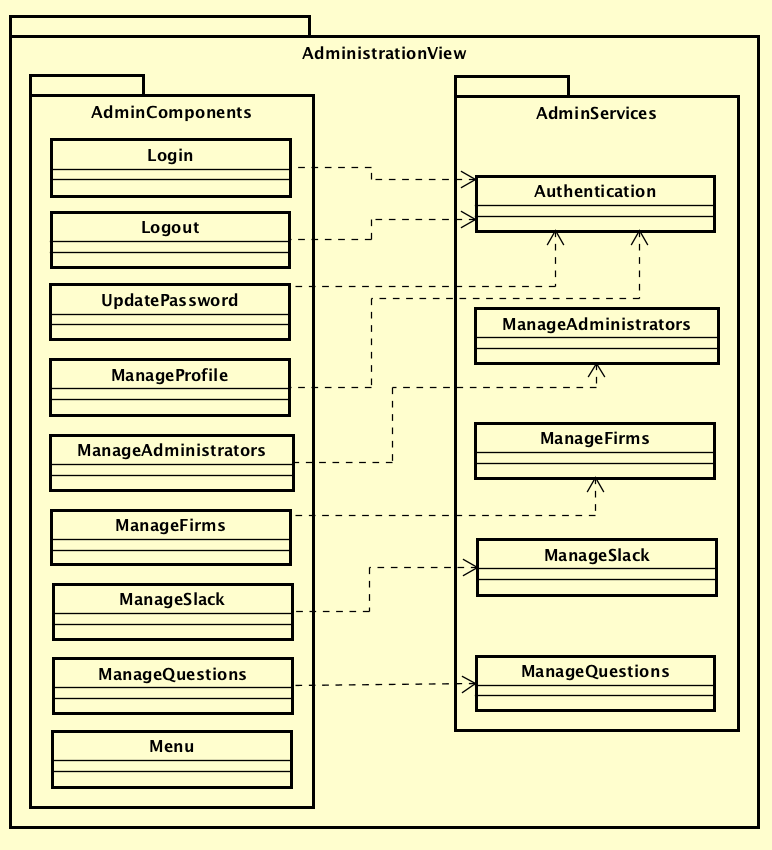
\includegraphics[scale=0.7]{Architettura/Front-End/Administration/AdministrationView.png}
				\caption{Schema del componente \texttt{Front-End :: AdministrationView}}
			\end{figure}
		\paragraph{Informazioni sul package}\begin{itemize}
		\item \textbf{Descrizione}: Package dedicato alla parte client dell'Admin e del SuperAdmin
		\item \textbf{Padre}: Front-End
		\item \textbf{Package contenuti}:
	\begin{itemize}\item AdministrationView :: AdminComponents: Classe contenente tutti i metodi necessari a gestire il Front-End della console amministrativa
	\item AdministrationView :: AdminServices: Package che fornisce tutti i servizi utilizzabili da un amministratore ed un super amministratore nella view del Front-End
	\end{itemize}\end{itemize}
	\subsubsection{ \texttt{Front-End :: AdministrationView :: AdminComponents}}
		\begin{figure}[!h]
			\centering
			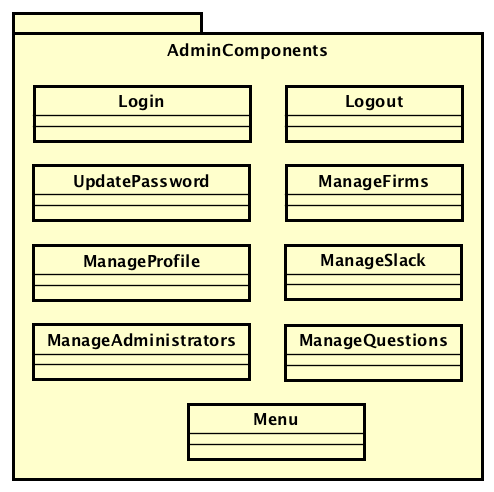
\includegraphics[scale=0.7]{Architettura/Front-End/Administration/AdminComponents.png}
			\caption{Schema del componente \texttt{Front-End :: AdministrationView :: AdminComponents}}
		\end{figure}

	\paragraph{Informazioni sul package}\begin{itemize}\item \textbf{Descrizione}: Classe contenente tutti i metodi necessari a gestire il Front-End della console amministrativa\item \textbf{Padre}: AdministrationView\item \textbf{Package contenuti}:
	\begin{itemize}\item AdministrationView :: AdminComponents :: Login: Componente che contiene al suo interno la sua view, il suo controller, ed i model di cui necessita
	\item AdministrationView :: AdminComponents :: Logout: Componente che contiene al suo interno la sua view, il suo controller, ed i model di cui necessita
	\item AdministrationView :: AdminComponents :: ManageAdministrators: Componente che contiene al suo interno la sua view, il suo controller, ed i model di cui necessita
	\item AdministrationView :: AdminComponents :: ManageFirms: Componente che contiene al suo interno la sua view, il suo controller, ed i model di cui necessita
	\item AdministrationView :: AdminComponents :: ManageProfile: Componente che contiene al suo interno la sua view, il suo controller, ed i model di cui necessita
	\item AdministrationView :: AdminComponents :: ManageQuestions: Componente che contiene al suo interno la sua view, il suo controller, ed i model di cui necessita
	\item AdministrationView :: AdminComponents :: ManageSlack: Componente che contiene al suo interno la sua view, il suo controller, ed i model di cui necessita
	\item AdministrationView :: AdminComponents :: Menu: Componente che contiene al suo interno la sua view, il suo controller, ed i model di cui necessita
	\item AdministrationView :: AdminComponents :: UpdatePassword: Componente che contiene al suo interno la sua view, il suo controller, ed i model di cui necessita
	\end{itemize}\end{itemize}
	\subsubsection{ \texttt{Front-End :: AdministrationView :: AdminComponents :: Login}}
		\begin{figure}[!h]
			\centering
			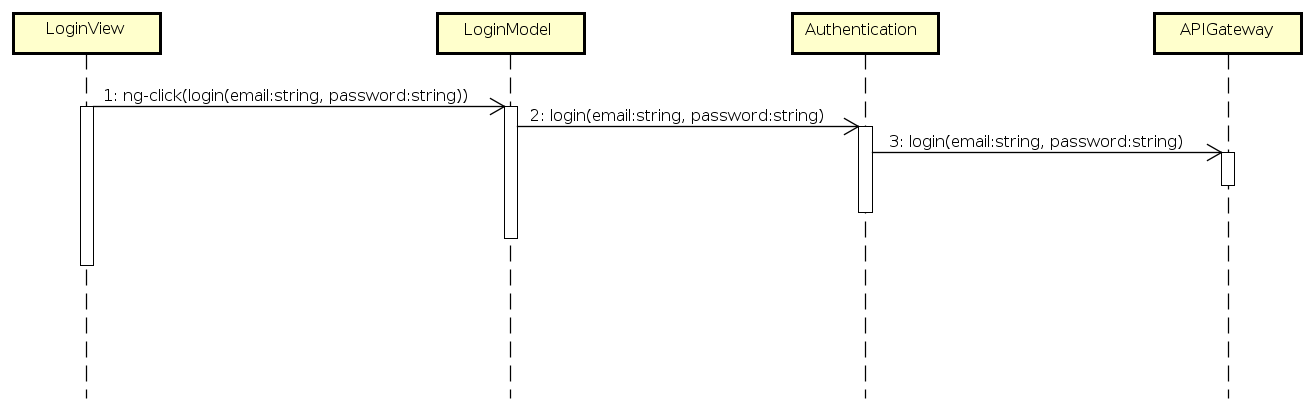
\includegraphics[scale=0.7]{Architettura/Front-End/Administration/AdminComponents/Login.png}
			\caption{Schema del componente \texttt{Front-End :: AdministrationView :: AdminComponents :: Login}}
		\end{figure}

	\paragraph{Informazioni sul package}\begin{itemize}\item \textbf{Descrizione}: Componente che contiene al suo interno la sua view, il suo controller, ed i model di cui necessita\item \textbf{Padre}: AdminComponents\paragraph{Classi}
	\subparagraph{\texttt{Front-End :: AdministrationView :: AdminComponents :: Login :: LoginController}}
	\begin{itemize}\item \textbf{Descrizione}: Controller che gestisce la view di LoginView permettendo ad un amministratore di effettuare l'accesso alla console amministrativa
	\item \textbf{Utilizzo}: il metodo verrà utilizzato per implementare l'accesso alla console amministrativa da parte di un Admin
	\item \textbf{Attributi}:
	\begin{itemize}
	\item \texttt{email: string}\

	 Attributo che rappresenta la email inserita dall'amministratore.
	\end{itemize}
	\begin{itemize}
	\item \texttt{password: string}\

	 Attributo che rappresenta la password inserita dall'amministratore.
	\end{itemize}
	\item \textbf{Metodi}:
	\begin{itemize}
	\item \texttt{login(email, password) : void}\

	 Funzione che permette all'amministratore di effettuare l'accesso alla console amministrativa

	\item \textbf{Argomenti}:
	\begin{itemize}
	\item \texttt{email : string}\

	 Parametro che indica la email inserita dall'amministratore.
	\item \texttt{password : string}\

	 Parametro che indica la password inserita dall'amministratore.
	\end{itemize}
	\end{itemize}\vspace{0.5em}
	\begin{itemize}
	\item \texttt{sendEmail(email) : void}\

	 Funzione che permette di inviare una email ad un amministratore che vuole ripristinare la sua password dimenticata

	\item \textbf{Argomenti}:
	\begin{itemize}
	\item \texttt{email : string}\

	 Parametro che indica la email inserita dall'amministratore.
	\end{itemize}
	\end{itemize}\vspace{0.5em}
	\end{itemize}

	\subparagraph{\texttt{Front-End :: AdministrationView :: AdminComponents :: Login :: LoginView}}
	\begin{itemize}\item \textbf{Descrizione}: View di Login, permette ad un amministratore di effettuare l'accesso alla console amministrativa
	\item \textbf{Utilizzo}: View di Login
	\end{itemize}\end{itemize}

	\newpage
	\subsubsection{ \texttt{Front-End :: AdministrationView :: AdminComponents :: Logout}}
		\begin{figure}[!h]
			\centering
			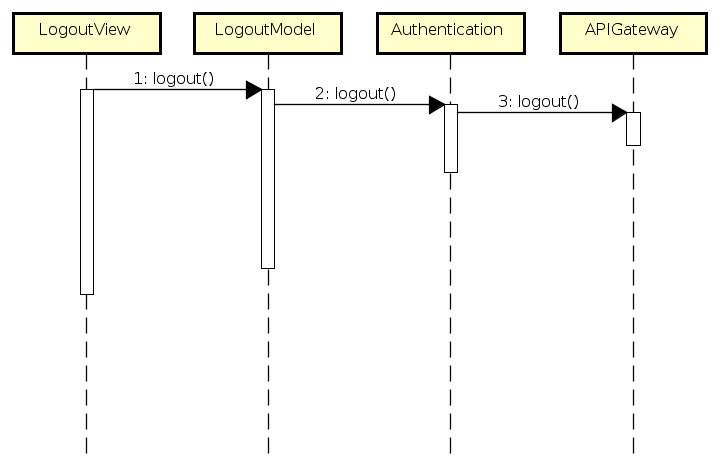
\includegraphics[scale=0.7]{Architettura/Front-End/Administration/AdminComponents/Logout.png}
			\caption{Schema del componente \texttt{Front-End :: AdministrationView :: AdminComponents :: Logout}}
		\end{figure}

	\paragraph{Informazioni sul package}\begin{itemize}\item \textbf{Descrizione}: Componente che contiene al suo interno la sua view, il suo controller, ed i model di cui necessita\item \textbf{Padre}: AdminComponents\paragraph{Classi}
	\subparagraph{\texttt{Front-End :: AdministrationView :: AdminComponents :: Logout :: LogoutController}}
	\begin{itemize}\item \textbf{Descrizione}: Compomente dedicato all'operazione di logout
	\item \textbf{Utilizzo}: Usato per il logout dall'appicazione durante una conversazione
	\item \textbf{Metodi}:
	\begin{itemize}
	\item \texttt{logout() : void}\

	 Funzione che permette ad un amministratore correttamente loggato nell'area amministrativa di effettuare il logout e terminare la sessione
	\end{itemize}\vspace{0.5em}
	\end{itemize}\subparagraph{\texttt{Front-End :: AdministrationView :: AdminComponents :: Logout :: LogoutView}}
	\begin{itemize}\item \textbf{Descrizione}: View del componente dedicato all'operazione di logout
	\item \textbf{Utilizzo}: View di Logout
	\end{itemize}\end{itemize}
	\subsubsection{ \texttt{Front-End :: AdministrationView :: AdminComponents :: ManageAdministrators}}
		\begin{figure}[!h]
			\centering
			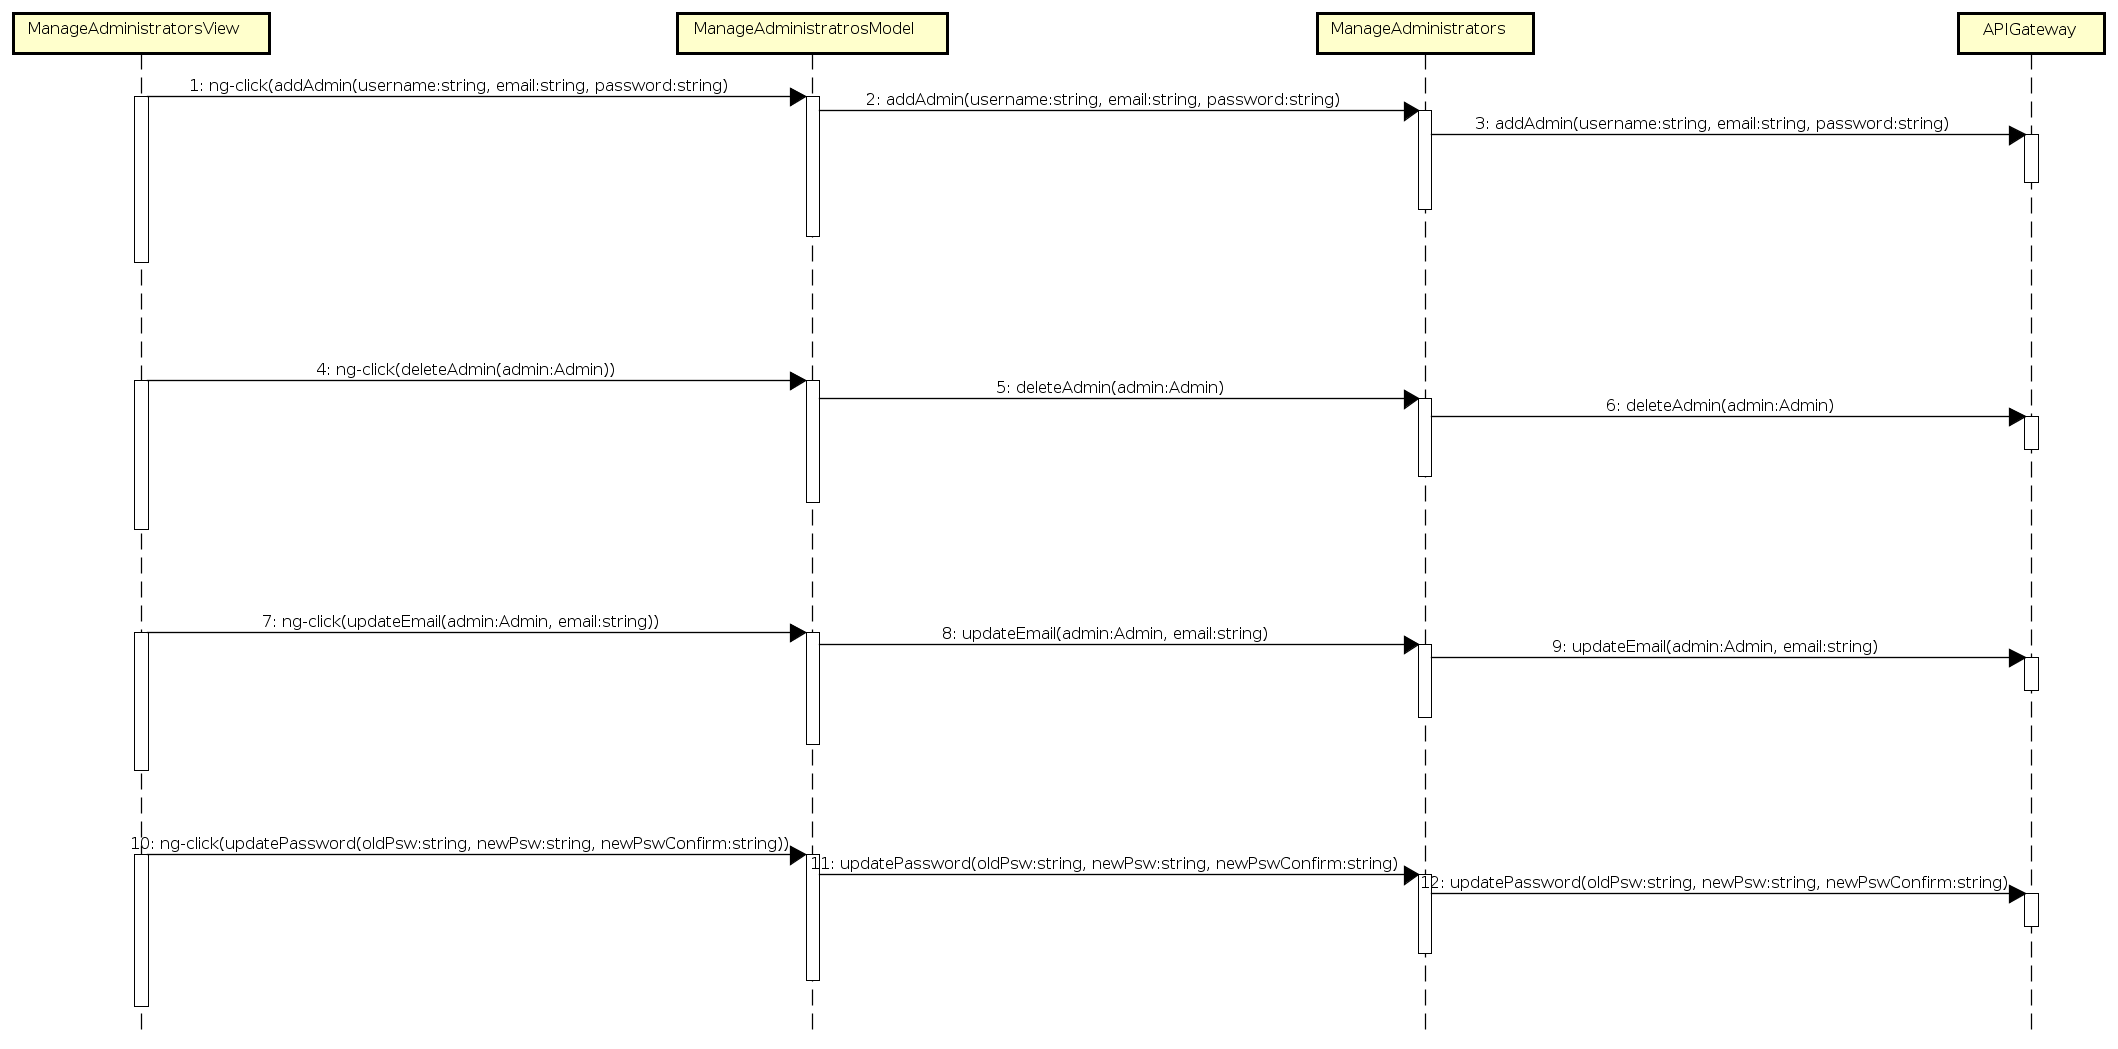
\includegraphics[scale=0.7]{Architettura/Front-End/Administration/AdminComponents/ManageAdministrators.png}
			\caption{Schema del componente \texttt{Front-End :: AdministrationView :: AdminComponents :: ManageAdministrators}}
		\end{figure}

	\paragraph{Informazioni sul package}\begin{itemize}\item \textbf{Descrizione}: Componente che contiene al suo interno la sua view, il suo controller, ed i model di cui necessita\item \textbf{Padre}: AdminComponents\paragraph{Classi}
	\subparagraph{\texttt{Front-End :: AdministrationView :: AdminComponents :: ManageAdministrators :: ManageAdministratorsController}}
	\begin{itemize}\item \textbf{Descrizione}: Controller che gestisce la view di ManageAdministrators permettendo ad un SuperAdmin di gestire le informazioni degli altri amministratori
	\item \textbf{Utilizzo}: Gestione degli amministratori
	\item \textbf{Attributi}:
	\begin{itemize}
	\item \texttt{admins: Admin[]}\

	 Attributo che indica gli amministratori presenti nel sistema.
	\end{itemize}
	\begin{itemize}
	\item \texttt{page\_id: int}\

	 Attributo che indica l'id della pagina corrente.
	\end{itemize}
	\item \textbf{Metodi}:
	\begin{itemize}
	\item \texttt{addAdmin(email, password, username) : void}\

	 Funzione che permette ad un amministratore super di aggiungere un nuovo amministratore al sistema

	\item \textbf{Argomenti}:
	\begin{itemize}
	\item \texttt{email : string}\

	 Parametro che indica la email dell'amministratore da aggiungere.
	\item \texttt{password : string}\

	 Parametro che indica la password del nuovo amministratore da aggiungere al sistema.
	\item \texttt{username : string}\

	 Parametro che indica il nuovo username dell'amministratore da aggiungere.
	\end{itemize}
	\end{itemize}\vspace{0.5em}
	\begin{itemize}
	\item \texttt{deleteAdmin(admin) : void}\

	 Funzione che permette ad un SuperAdmin di eliminare un Admin dal sistema

	\item \textbf{Argomenti}:
	\begin{itemize}
	\item \texttt{admin : Admin}\

	 Parametro che indica l'amministratore da rimuovere.
	\end{itemize}
	\end{itemize}\vspace{0.5em}
	\begin{itemize}
	\item \texttt{updatePassword(newPsw, newPswConfirm, oldPsw) : void}\

	 Funzione che permette ad un SuperAdmin di modificare la password di un Admin presente nel sistema

	\item \textbf{Argomenti}:
	\begin{itemize}
	\item \texttt{newPsw : string}\

	 Parametro che indica la nuova password inserita dall'amministratore.
	\item \texttt{newPswConfirm : string}\

	 Parametro che indica la conferma della nuova password inserita dall'amministratore.
	\item \texttt{oldPsw : string}\

	 Parametro che indica la vecchia password inserita dall'amministratore.
	\end{itemize}
	\end{itemize}\vspace{0.5em}
	\begin{itemize}
	\item \texttt{updateEmail(admin) : void}\

	 Funzione che permette ad un SuperAdmin di modificare la email di un Admin presente nel sistema

	\item \textbf{Argomenti}:
	\begin{itemize}
	\item \texttt{admin : Admin}\

	 Parametro che indica l'amministratore da modificare.
	\end{itemize}
	\end{itemize}\vspace{0.5em}
	\end{itemize}\subparagraph{\texttt{Front-End :: AdministrationView :: AdminComponents :: ManageAdministrators :: ManageAdministratorsView}}
	\begin{itemize}\item \textbf{Descrizione}: View di ManageAdministrators, permette ad un SuperAdmin di gestire le informazioni degli altri amministratori
	\item \textbf{Utilizzo}: View di ManageAdministrators
	\end{itemize}\end{itemize}

	\newpage
	\subsubsection{ \texttt{Front-End :: AdministrationView :: AdminComponents :: ManageFirms}}
		\begin{figure}[!h]
			\centering
			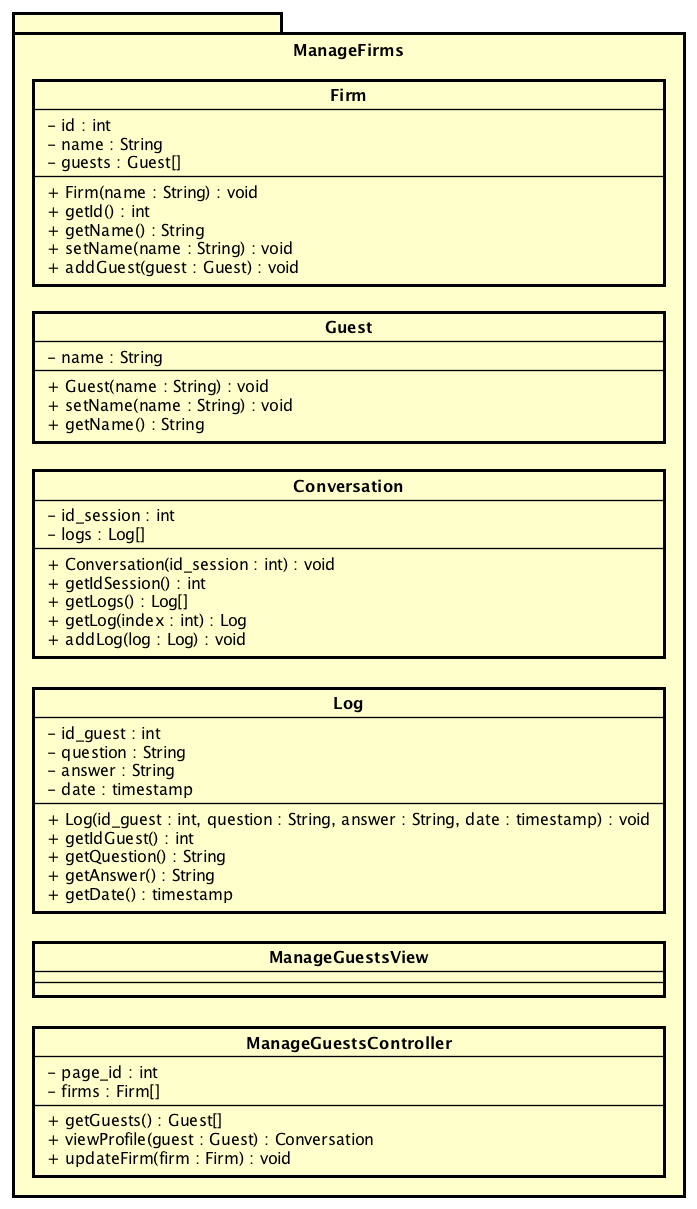
\includegraphics[scale=0.5]{Architettura/Front-End/Administration/AdminComponents/ManageFirms.png}
			\caption{Schema del componente \texttt{Front-End :: AdministrationView :: AdminComponents :: ManageFirms}}
		\end{figure}

	\paragraph{Informazioni sul package}\begin{itemize}\item \textbf{Descrizione}: Componente che contiene al suo interno la sua view, il suo controller, ed i model di cui necessita\item \textbf{Padre}: AdminComponents\paragraph{Classi}
	\subparagraph{\texttt{Front-End :: AdministrationView :: AdminComponents :: ManageFirms :: ManageFirmsController}}
	\begin{itemize}\item \textbf{Descrizione}: Componente utilizzato per la gestione degli oggetti di tipo Firm
	\item \textbf{Utilizzo}: Componente utilizzato per la gestione degli oggetti che modellano l'azienda
	\item \textbf{Attributi}:
	\begin{itemize}
	\item \texttt{firms: Firm[]}\

	 Attributo che indica le aziende di tipo Firm presenti nel sistema.
	\end{itemize}
	\begin{itemize}
	\item \texttt{page\_id: int}\

	 Attributo che indica l'id della pagina corrente.
	\end{itemize}
	\item \textbf{Metodi}:
	\begin{itemize}
	\item \texttt{getGuest() : Guest}\

	 Funzione che ritorna tutti gli ospiti registrati ad una determinata azienda
	\end{itemize}\vspace{0.5em}
	\begin{itemize}
	\item \texttt{updateFirm(firm) : void}\

	 Funzione che aggiorna un azienda intera, compresi gli ospiti associati ad essa

	\item \textbf{Argomenti}:
	\begin{itemize}
	\item \texttt{firm : Firm}\

	 Parametro che indica l'azienda da aggiornare .
	\end{itemize}
	\end{itemize}\vspace{0.5em}
	\begin{itemize}
	\item \texttt{viewProfile(guest) : Conversation}\

	 Funzione che ritorna l'intera conversazione di un ospite

	\item \textbf{Argomenti}:
	\begin{itemize}
	\item \texttt{guest : Guest}\

	 Parametro che indica l'ospite di cui si vuole avere l'intera conversazione.
	\end{itemize}
	\end{itemize}\vspace{0.5em}
	\end{itemize}\subparagraph{\texttt{Front-End :: AdministrationView :: AdminComponents :: ManageFirms :: ManageFirmsView}}
	\begin{itemize}\item \textbf{Descrizione}: View utilizzata per la scelta degli oggetti di tipo Firm
	\item \textbf{Utilizzo}: View di ManageFirms
	\end{itemize}\end{itemize}

	\newpage
	\subsubsection{ \texttt{Front-End :: AdministrationView :: AdminComponents :: ManageProfile}}
		\begin{figure}[!h]
			\centering
			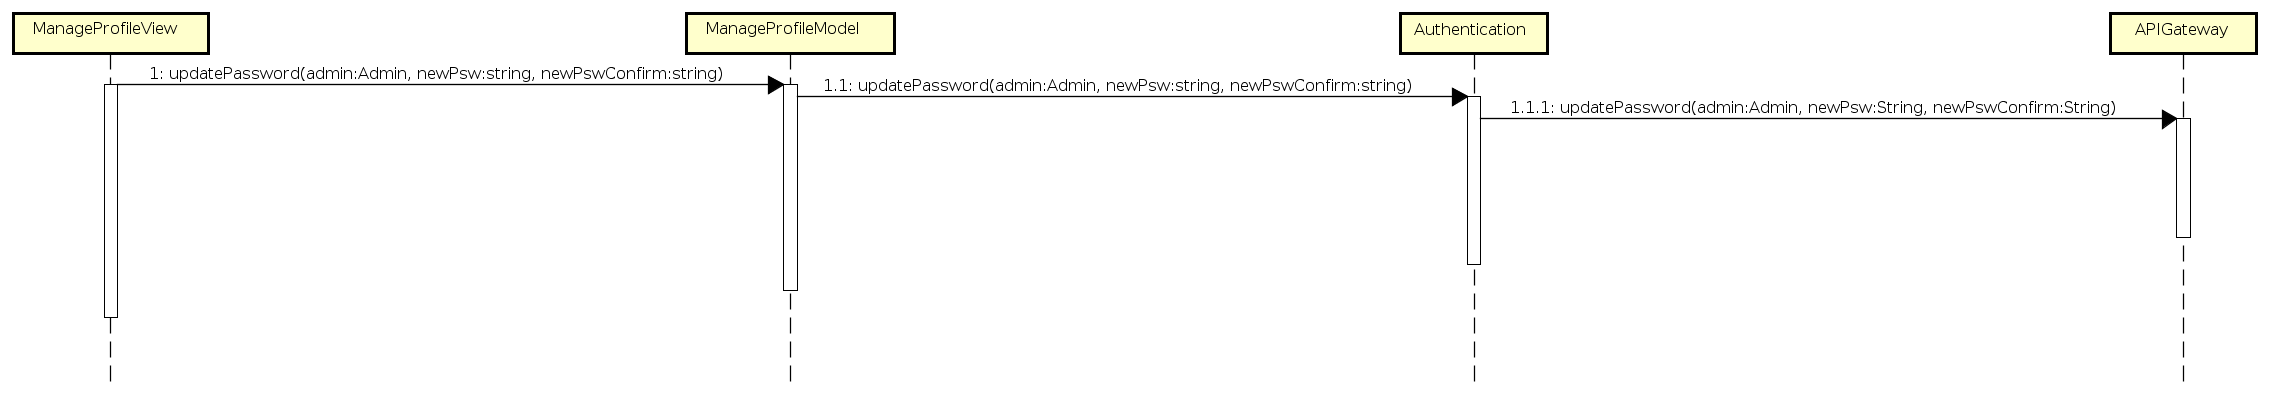
\includegraphics[scale=0.7]{Architettura/Front-End/Administration/AdminComponents/ManageProfile.png}
			\caption{Schema del componente \texttt{Front-End :: AdministrationView :: AdminComponents :: ManageProfile}}
		\end{figure}

	\paragraph{Informazioni sul package}\begin{itemize}\item \textbf{Descrizione}: Componente che contiene al suo interno la sua view, il suo controller, ed i model di cui necessita\item \textbf{Padre}: AdminComponents\paragraph{Classi}
	\subparagraph{\texttt{Front-End :: AdministrationView :: AdminComponents :: ManageProfile :: ManageProfile}}
	\begin{itemize}\item \textbf{Descrizione}: View di ManageProfile, permette ad un amministratore di gestire il proprio profilo nell'area amministrativa
	\item \textbf{Utilizzo}: View di ManageProfile
	\end{itemize}\subparagraph{\texttt{Front-End :: AdministrationView :: AdminComponents :: ManageProfile :: ManageProfileController}}
	\begin{itemize}\item \textbf{Descrizione}: Controller che gestisce la view di ManageProfileView permettendo ad un amministratore di gestire il proprio profilo nell'area amministrativa
	\item \textbf{Utilizzo}: Verrà utilizzata dall'admin per la gestione del proprio profilo
	\item \textbf{Attributi}:
	\begin{itemize}
	\item \texttt{email: string}\

	 Attributo che indica la email dell'amministratore.
	\end{itemize}
	\begin{itemize}
	\item \texttt{page\_id: int}\

	 Attributo che indica l'id della pagina corrente.
	\end{itemize}
	\begin{itemize}
	\item \texttt{password: string}\

	 Attributo che indica la password dell'amministratore.
	\end{itemize}
	\item \textbf{Metodi}:
	\begin{itemize}
	\item \texttt{updatePassword(admin, newPsw, newPswConfirm) : void}\

	 Funzione che permette ad un amministratore di aggiornare la propria password

	\item \textbf{Argomenti}:
	\begin{itemize}
	\item \texttt{admin : Admin}\

	 Parametro che indica l'amministratore corrente.
	\item \texttt{newPsw : string}\

	 Parametro che indica la nuova password inserita dall'amministratore.
	\item \texttt{newPswConfirm : string}\

	 Parametro che indica la conferma della nuova password inserita dall'amministratore.
	\end{itemize}
	\end{itemize}\vspace{0.5em}
	\end{itemize}\subparagraph{\texttt{Front-End :: AdministrationView :: AdminComponents :: ManageProfile :: ManageProfileView}}
	\begin{itemize}\item \textbf{Descrizione}: View di ManageProfile, permette ad un amministratore di gestire il proprio profilo nell'area amministrativa
	\item \textbf{Utilizzo}: View di ManageProfile
	\end{itemize}\end{itemize}

	\newpage
	\subsubsection{ \texttt{Front-End :: AdministrationView :: AdminComponents :: ManageQuestions}}
		\begin{figure}[!h]
			\centering
			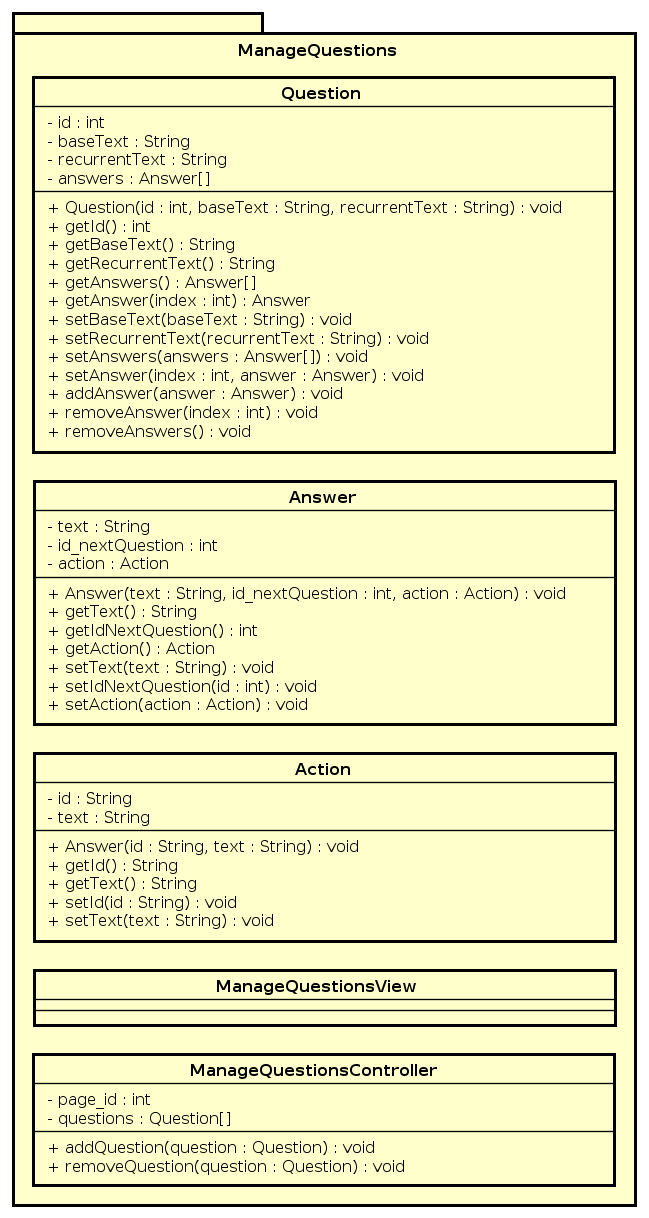
\includegraphics[scale=0.5]{Architettura/Front-End/Administration/AdminComponents/ManageQuestions.png}
			\caption{Schema del componente \texttt{Front-End :: AdministrationView :: AdminComponents :: ManageQuestions}}
		\end{figure}

	\paragraph{Informazioni sul package}\begin{itemize}\item \textbf{Descrizione}: Componente che contiene al suo interno la sua view, il suo controller, ed i model di cui necessita\item \textbf{Padre}: AdminComponents\paragraph{Classi}
	\subparagraph{\texttt{Front-End :: AdministrationView :: AdminComponents :: ManageQuestions :: ManageQuestionsController}}
	\begin{itemize}\item \textbf{Descrizione}: Componente per le domande e interazioni
	\item \textbf{Utilizzo}: Componente utilizzato per le domande e interazioni
	\item \textbf{Attributi}:
	\begin{itemize}
	\item \texttt{page\_id: int}\

	 Attributo che indica l'id della pagina corrente
	.
	\end{itemize}
	\begin{itemize}
	\item \texttt{questions: Question[]}\

	 Parametro che indica la lista delle domande presenti nel sistema.
	\end{itemize}
	\item \textbf{Metodi}:
	\begin{itemize}
	\item \texttt{addQuestion(question) : void}\

	 Funzione che permette di aggiungere una nuova domanda al sistema

	\item \textbf{Argomenti}:
	\begin{itemize}
	\item \texttt{question : Question}\

	 Parametro che indica la domanda da aggiungere al sistema.
	\end{itemize}
	\end{itemize}\vspace{0.5em}
	\begin{itemize}
	\item \texttt{removeQuestion(question) : void}\

	 Funzione che permette di rimuovere una domanda dal sistema

	\item \textbf{Argomenti}:
	\begin{itemize}
	\item \texttt{question : Question}\

	 Parametro che indica la domanda da rimuovere dal sistema.
	\end{itemize}
	\end{itemize}\vspace{0.5em}
	\end{itemize}\subparagraph{\texttt{Front-End :: AdministrationView :: AdminComponents :: ManageQuestions :: ManageQuestionsView}}
	\begin{itemize}\item \textbf{Descrizione}: View per la gestione di domande e interazioni
	\item \textbf{Utilizzo}: View di ManageQuesitons
	\end{itemize}\end{itemize}

	\newpage
	\subsubsection{ \texttt{Front-End :: AdministrationView :: AdminComponents :: ManageSlack}}
		\begin{figure}[!h]
			\centering
			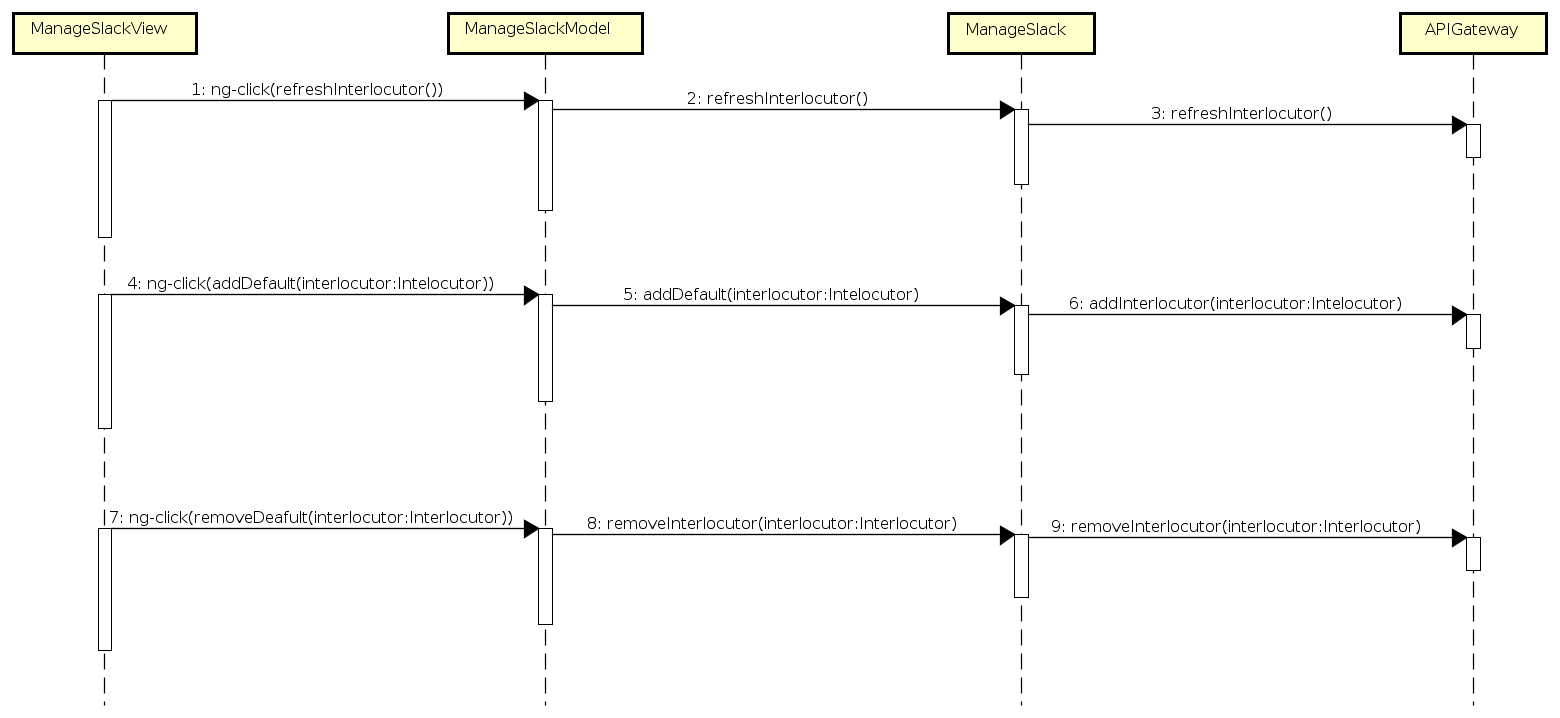
\includegraphics[scale=0.5]{Architettura/Front-End/Administration/AdminComponents/ManageSlack.png}
			\caption{Schema del componente \texttt{Front-End :: AdministrationView :: AdminComponents :: ManageSlack}}
		\end{figure}

	\paragraph{Informazioni sul package}\begin{itemize}\item \textbf{Descrizione}: Componente che contiene al suo interno la sua view, il suo controller, ed i model di cui necessita\item \textbf{Padre}: AdminComponents\paragraph{Classi}
	\subparagraph{\texttt{Front-End :: AdministrationView :: AdminComponents :: ManageSlack :: ManageSlackController}}
	\begin{itemize}\item \textbf{Descrizione}: Componente per la gestione dei canali Slack
	\item \textbf{Utilizzo}: Componente per la gestione dei canali Slack
	\item \textbf{Attributi}:
	\begin{itemize}
	\item \texttt{defaultInterlocutors: Interlocutor[]}\

	 Attributo che indica gli interlocutori presenti nel sistema che fanno parte della lista di default del canale \#azienda.
	\end{itemize}
	\begin{itemize}
	\item \texttt{interlocutor: Interlocutor[]}\

	 Attributo che indica gli interlocutori presenti nel sistema.
	\end{itemize}
	\begin{itemize}
	\item \texttt{page\_id: int}\

	 Attributo che indica l'id della pagina corrente.
	\end{itemize}
	\item \textbf{Metodi}:
	\begin{itemize}
	\item \texttt{addDefault(interlocutor) : void}\

	 Funzione che permette di aggiungere un interlocutore alla lista di default \#azienda

	\item \textbf{Argomenti}:
	\begin{itemize}
	\item \texttt{interlocutor : Interlocutor}\

	 Parametro che indica l'interlocutore da associare alla lista di default.
	\end{itemize}
	\end{itemize}\vspace{0.5em}
	\begin{itemize}
	\item \texttt{refreshInterlocutors() : void}\

	 Funzione che permette di aggiornare gli interlocutori presenti nel sistema prelevandoli dal team Slack dell'azienda
	\end{itemize}\vspace{0.5em}
	\begin{itemize}
	\item \texttt{removeDafault(Interlocutor) : void}\

	 Funzione che permette di rimuovere un interlocutore alla lista di default \#azienda

	\item \textbf{Argomenti}:
	\begin{itemize}
	\item \texttt{Interlocutor : Interlocutor}\

	 Parametro che indica l'interlocutore da disassociare alla lista di default.
	\end{itemize}
	\end{itemize}\vspace{0.5em}
	\end{itemize}\subparagraph{\texttt{Front-End :: AdministrationView :: AdminComponents :: ManageSlack :: ManageSlackView}}
	\begin{itemize}\item \textbf{Descrizione}: View del componente per la gestione dei canali Slack
	\item \textbf{Utilizzo}: View di ManageSlack
	\end{itemize}\end{itemize}

	\subsubsection{ \texttt{Front-End :: AdministrationView :: AdminComponents :: Menu}}
		\begin{figure}[!h]
			\centering
			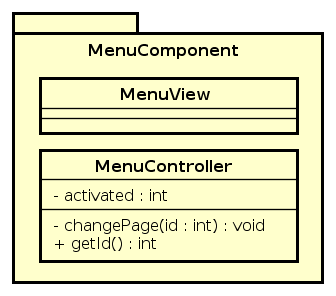
\includegraphics[scale=0.7]{Architettura/Front-End/Administration/AdminComponents/Menu.png}
			\caption{Schema del componente \texttt{Front-End :: AdministrationView :: AdminComponents :: Menu}}
		\end{figure}

	\paragraph{Informazioni sul package}\begin{itemize}\item \textbf{Descrizione}: Componente che contiene al suo interno la sua view, il suo controller, ed i model di cui necessita\item \textbf{Padre}: AdminComponents\paragraph{Classi}
	\subparagraph{\texttt{Front-End :: AdministrationView :: AdminComponents :: Menu :: MenuController}}
	\begin{itemize}\item \textbf{Descrizione}: Controller che gestisce la view di MenuComponent permettendo di gestire il menu dell'area amministrativa
	\item \textbf{Utilizzo}: Verrà utilizzato dall'Admin per gestire il menu dell'area amministrativa
	\item \textbf{Attributi}:
	\begin{itemize}
	\item \texttt{activated: int}\

	 Attributo che indica l'id della pagina attiva.
	\end{itemize}
	\item \textbf{Metodi}:
	\begin{itemize}
	\item \texttt{changePage(id) : void}\

	 Funzione che permette di cambiare pagina in base all'id di quella richiesta

	\item \textbf{Argomenti}:
	\begin{itemize}
	\item \texttt{id : int}\

	 Parametro che indica l'id della nuova pagina richiesta.
	\end{itemize}
	\end{itemize}\vspace{0.5em}
	\end{itemize}\subparagraph{\texttt{Front-End :: AdministrationView :: AdminComponents :: Menu :: MenuView}}
	\begin{itemize}\item \textbf{Descrizione}: View di MenuComponent, permette di gestire il menu dell'area amministrativa
	\item \textbf{Utilizzo}: View di Menu
	\end{itemize}\end{itemize}

	\newpage
	\subsubsection{ \texttt{Front-End :: AdministrationView :: AdminComponents :: UpdatePassword}}
		\begin{figure}[!h]
			\centering
			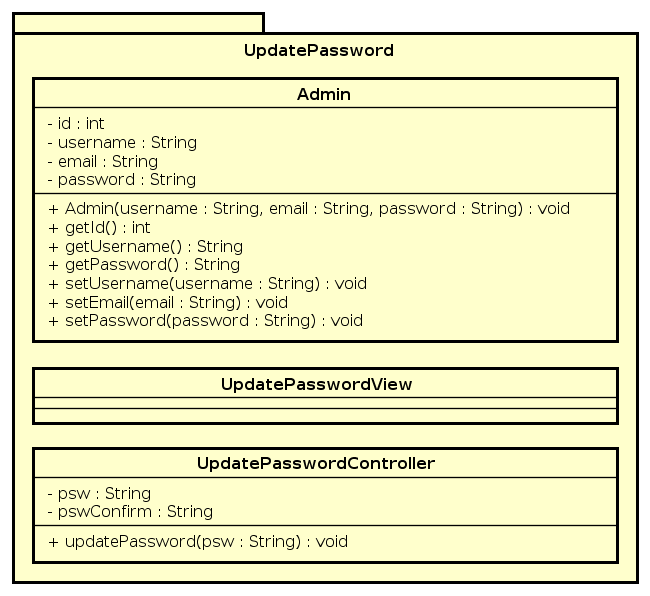
\includegraphics[scale=0.7]{Architettura/Front-End/Administration/AdminComponents/UpdatePassword.png}
			\caption{Schema del componente \texttt{Front-End :: AdministrationView :: AdminComponents :: UpdatePassword}}
		\end{figure}

	\paragraph{Informazioni sul package}\begin{itemize}\item \textbf{Descrizione}: Componente che contiene al suo interno la sua view, il suo controller, ed i model di cui necessita\item \textbf{Padre}: AdminComponents\paragraph{Classi}
	\subparagraph{\texttt{Front-End :: AdministrationView :: AdminComponents :: UpdatePassword :: UpdatePasswordController}}
	\begin{itemize}\item \textbf{Descrizione}: Controller che gestisce la view di UpdatePasswordView permettendo ad un amministratore di effettuare l'aggiornamento della propria password previa email ricevuta nella propria casella di posta
	\item \textbf{Utilizzo}: Metodo utilizzato per gestire il cambio della propria password da parte di un Admin
	\item \textbf{Attributi}:
	\begin{itemize}
	\item \texttt{password: string}\

	 Attributo che indica la password inserita dall'amministratore.
	\end{itemize}
	\begin{itemize}
	\item \texttt{passwordConfirm: string}\

	 Attributo che indica la password inserita dall'amministratore una seconda volta per conferma.
	\end{itemize}
	\item \textbf{Metodi}:
	\begin{itemize}
	\item \texttt{updatePassword(psw) : void}\

	 Funzione che permette all'amministratore di aggiornare la propria password

	\item \textbf{Argomenti}:
	\begin{itemize}
	\item \texttt{psw : string}\

	 Parametro che indica la nuova password inserita dall'amministratore.
	\end{itemize}
	\end{itemize}\vspace{0.5em}
	\end{itemize}\subparagraph{\texttt{Front-End :: AdministrationView :: AdminComponents :: UpdatePassword :: UpdatePasswordView}}
	\begin{itemize}\item \textbf{Descrizione}: View di UpdatePassword, permette ad un amministratore di effettuare l'aggiornamento della propria password previa email ricevuta nella propria casella di posta
	\item \textbf{Utilizzo}: View di UpdatePasword
	\end{itemize}\end{itemize}

	\newpage
	\subsubsection{ \texttt{Front-End :: AdministrationView :: AdminServices}}
	\begin{figure}[!h]
		\centering
		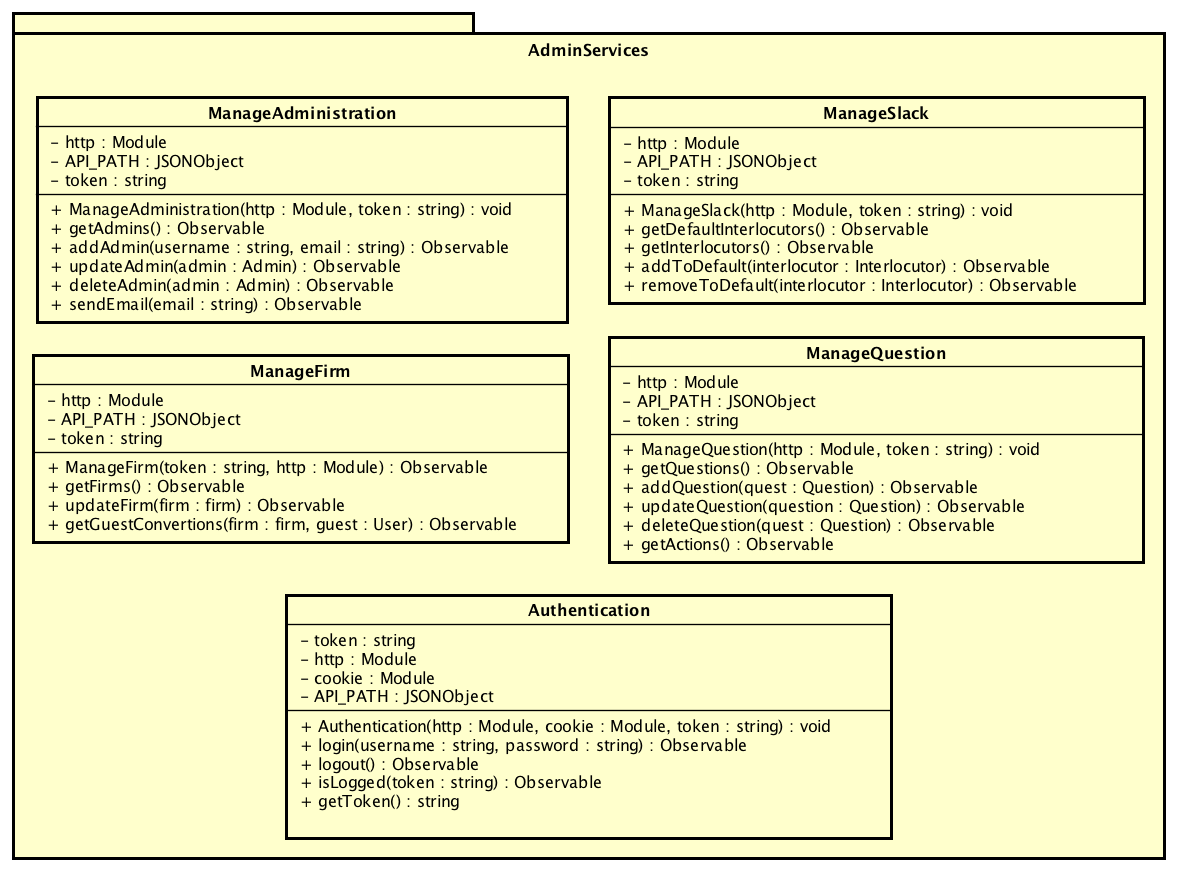
\includegraphics[width=\textwidth]{Architettura/Front-End/Administration/AdministrationServices.png}
		\caption{Schema del componente \texttt{Front-End :: AdministrationView :: AdminServices}}
	\end{figure}
	\paragraph{Informazioni sul package}\begin{itemize}\item \textbf{Descrizione}: Package che fornisce tutti i servizi utilizzabili da un amministratore ed un super amministratore nella view del Front-End\item \textbf{Padre}: AdministrationView\paragraph{Classi}
	\subparagraph{\texttt{Front-End :: AdministrationView :: AdminServices :: ManageAdministrators}}
	\begin{itemize}\item \textbf{Descrizione}: Servizi per i componenti del client dell'Admin e del SuperAdmin.
	\item \textbf{Utilizzo}: Gestione servizi Admin e SuperAdmin.
	\item \textbf{Attributi}:
	\begin{itemize}
	\item \texttt{-API\_PATH: JSONObject}\

	 Attributo che rappresenta il percorso per le API in formato JSON.
	\end{itemize}
	\begin{itemize}
	\item \texttt{-http: Module}\

	 Attributo che rappresenta il modulo per la connessione http.
	\end{itemize}
	\begin{itemize}
	\item \texttt{-token: string}\

	 Stringa che contiene il token.
	\end{itemize}
	\item \textbf{Metodi}:
	\begin{itemize}
	\item \texttt{addAdmin(email, username) : Observable}\

	 Aggiunge un Admin con i realativi dati di username ed e-mail. L'observable di ritorno serve ad indicare la presenza di errori o meno

	\item \textbf{Argomenti}:
	\begin{itemize}
	\item \texttt{email : string}\

	 Email del nuovo Admin.
	\item \texttt{username : string}\

	 Nome del nuovo Admin.
	\end{itemize}
	\end{itemize}\vspace{0.5em}
	\begin{itemize}
	\item \texttt{deleteAdmin(admin) : Observable}\

	 Elimina l'Admin passato come parametro di ingresso. L'oggetto observable serve per il controllo degli errori

	\item \textbf{Argomenti}:
	\begin{itemize}
	\item \texttt{admin : Admin}\

	 Parametro che contiene i dati di un ammnistratore.
	\end{itemize}
	\end{itemize}\vspace{0.5em}
	\begin{itemize}
	\item \texttt{getAdmins() : Observable}\

	 Restituisce l'observable di tutti gli Admin
	\end{itemize}\vspace{0.5em}
	\begin{itemize}
	\item \texttt{ManageAdministration(token) : void}\

	 Costruttore della classe.

	\item \textbf{Argomenti}:
	\begin{itemize}
	\item \texttt{token : string}\

	 Stringa che contiene il token.
	\end{itemize}
	\end{itemize}\vspace{0.5em}
	\begin{itemize}
	\item \texttt{sendEmail(email) : Observable}\

	 Metodo per inviare una email

	\item \textbf{Argomenti}:
	\begin{itemize}
	\item \texttt{email : string}\

	 Stringa contenete il testo di una email.
	\end{itemize}
	\end{itemize}\vspace{0.5em}
	\begin{itemize}
	\item \texttt{updateAdmin(admin) : Observable}\

	 Aggiorna un amministratore

	\item \textbf{Argomenti}:
	\begin{itemize}
	\item \texttt{admin : Admin}\

	 Contiene tutti i dati di un Admin.
	\end{itemize}
	\end{itemize}\vspace{0.5em}
	\item \textbf{Relazioni con altre classi}:
	\begin{itemize}
	\item \texttt{Back-End :: DatabaseInteraction :: DatabaseInteraction}: Classe che si occupa della connessione con il database e delle operazioni di lettura e scrittura.
	\end{itemize}
	\end{itemize}\subparagraph{\texttt{Front-End :: AdministrationView :: AdminServices :: ManageFirm}}
	\begin{itemize}\item \textbf{Descrizione}: Gestione servizi per i componenti client che si occupano delle aziende.
	\item \textbf{Utilizzo}: Utilizzato per gestire le aziende.
	\item \textbf{Attributi}:
	\begin{itemize}
	\item \texttt{-API\_PATH: JSONObject}\

	 Attributo che rappresenta il percorso per le API in formato JSON.
	\end{itemize}
	\begin{itemize}
	\item \texttt{-http: Module}\

	 Attributo che rappresenta il modulo per la connessione http.
	\end{itemize}
	\begin{itemize}
	\item \texttt{-token: string}\

	 Stringa che contiene il token.
	\end{itemize}
	\item \textbf{Metodi}:
	\begin{itemize}
	\item \texttt{getFirms() : Observable}\

	 Metodo che restituisce tutte le aziende tramite un oggetto di tipo Observable
	\end{itemize}\vspace{0.5em}
	\begin{itemize}
	\item \texttt{getGuestConvertions(firm, guest) : Observable}\

	 Metodo che fornisce l'intera conversazione di un ospite che lavora per una certa azienda

	\item \textbf{Argomenti}:
	\begin{itemize}
	\item \texttt{firm : Firm}\

	 Parametro che indica l'azienda per la quale un ospite lavora.
	\item \texttt{guest : User}\

	 Parametro che indica l'ospite per il quale si vuole estrapolare la conversazione .
	\end{itemize}
	\end{itemize}\vspace{0.5em}
	\begin{itemize}
	\item \texttt{ManageFirms(http, token) : Observable}\

	 Costruttore della classe che costruisce l'oggetto tramite un token di tipo stringa che identifica l'azienda e modulo per la connessione http

	\item \textbf{Argomenti}:
	\begin{itemize}
	\item \texttt{http : Module}\

	 Parametro che rappresenta il modulo di connessione http.
	\item \texttt{token : string}\

	 Parametro stringa che contiene il token che identifica l'azienda.
	\end{itemize}
	\end{itemize}\vspace{0.5em}
	\begin{itemize}
	\item \texttt{updateFirm(firm) : Observable}\

	 Metodo che permette di modificare uno specifico oggetto Firm che rappresenta un' azienda

	\item \textbf{Argomenti}:
	\begin{itemize}
	\item \texttt{firm : Firm}\

	 Parametro di tipo Firm che indica l'azienda che si vuole modificare .
	\end{itemize}
	\end{itemize}\vspace{0.5em}
	\item \textbf{Relazioni con altre classi}:
	\begin{itemize}
	\item \texttt{Back-End :: DatabaseInteraction :: DatabaseInteraction}: Classe che si occupa della connessione con il database e delle operazioni di lettura e scrittura.
	\end{itemize}
	\end{itemize}\subparagraph{\texttt{Front-End :: AdministrationView :: AdminServices :: ManageQuestion}}
	\begin{itemize}\item \textbf{Descrizione}: Classe che fornisce funzionalità per la gestione delle domande e delle interazioni collegate ad esse
	\item \textbf{Utilizzo}: Utilizzata per operazioni di gestione delle domande e relative interazioni
	\item \textbf{Attributi}:
	\begin{itemize}
	\item \texttt{API\_PATH: JSONObject}\

	 Attributo che rappresenta il percorso per le API in formato JSON.
	\end{itemize}
	\begin{itemize}
	\item \texttt{http: Module}\

	 Attributo che rappresenta il modulo per la connessione http.
	\end{itemize}
	\begin{itemize}
	\item \texttt{token: string}\

	 Stringa che contiene il token.
	\end{itemize}
	\item \textbf{Metodi}:
	\begin{itemize}
	\item \texttt{addQuestion(quest) : Observable}\

	 Metodo che aggiunge una domanda

	\item \textbf{Argomenti}:
	\begin{itemize}
	\item \texttt{quest : Question}\

	 Parametro di tipo Question che rappresenta la domanda da aggiungere
	\end{itemize}
	\end{itemize}\vspace{0.5em}
	\begin{itemize}
	\item \texttt{deleteQuestion(quest) : Observable}\

	 Metodo che permette di eliminare una domanda da quelle già presenti

	\item \textbf{Argomenti}:
	\begin{itemize}
	\item \texttt{quest : Question}\

	 Parametro di tipo Question che rappresenta la domanda che si intende eliminare
	\end{itemize}
	\end{itemize}\vspace{0.5em}
	\begin{itemize}
	\item \texttt{getActions() : Observable}\

	 Metodo che fornisce tutte le azioni possibili collegate alle domande disponibili sotto forma di un oggetto di tipo Observable
	\end{itemize}\vspace{0.5em}
	\begin{itemize}
	\item \texttt{getQuestions() : Observable}\

	 Metodo che fornisce tutte le domande disponibili sotto forma di un oggetto di tipo Observable
	\end{itemize}\vspace{0.5em}
	\begin{itemize}
	\item \texttt{ManageQuestion(http, token) : void}\

	 Costruttore della classe

	\item \textbf{Argomenti}:
	\begin{itemize}
	\item \texttt{http : Module}\

	 Parametro che rappresenta il modulo di connessione http passato per creare un oggetto di tipo ManageQuestion.
	\item \texttt{token : string}\

	 Parametro stringa che rappresenta il token passato per costruire un oggetto di tipo ManageQuestion.
	\end{itemize}
	\end{itemize}\vspace{0.5em}
	\begin{itemize}
	\item \texttt{updateQuestion(question) : Observable}\

	 Metodo che permette di aggiornare una domanda già esistente

	\item \textbf{Argomenti}:
	\begin{itemize}
	\item \texttt{question : Question}\

	 Parametro di tipo Question che rappresenta la domanda da aggiornare.
	\end{itemize}
	\end{itemize}\vspace{0.5em}
	\item \textbf{Relazioni con altre classi}:
	\begin{itemize}
	\item \texttt{Back-End :: DatabaseInteraction :: DatabaseInteraction}: Classe che si occupa della connessione con il database e delle operazioni di lettura e scrittura.
	\end{itemize}
	\end{itemize}\subparagraph{\texttt{Front-End :: AdministrationView :: AdminServices :: ManageSlack}}
	\begin{itemize}\item \textbf{Descrizione}: Gestione servizi lato client dei componenti che si interfacciano ai servizi di Slack.
	\item \textbf{Utilizzo}: Utilizzato per gestire i servizi di interfaccia ai servizi di Slack.
	\item \textbf{Attributi}:
	\begin{itemize}
	\item \texttt{-API\_PATH: JSONObject}\

	 Attributo che rappresenta il percorso per le API in formato JSON.
	\end{itemize}
	\begin{itemize}
	\item \texttt{-http: Module}\

	 Attributo che rappresenta il modulo per la connessione http.
	\end{itemize}
	\begin{itemize}
	\item \texttt{-token: string}\

	 Stringa che contiene il token.
	\end{itemize}
	\item \textbf{Metodi}:
	\begin{itemize}
	\item \texttt{addToDefault(interlocutor) : Observable}\

	 Aggiunge un interlocutore agli interlocutori di default

	\item \textbf{Argomenti}:
	\begin{itemize}
	\item \texttt{interlocutor : Interlocutor}\

	 Attributo che contiene un interlocutore.
	\end{itemize}
	\end{itemize}\vspace{0.5em}
	\begin{itemize}
	\item \texttt{getDefaultInterlocutors() : Observable}\

	 Metodo che restituisce gli interlocutori di default dei canali
	\end{itemize}\vspace{0.5em}
	\begin{itemize}
	\item \texttt{getInterlocutors() : Observable}\

	 Metodo che ritorna tutti gli interlocutori presenti nel Database
	\end{itemize}\vspace{0.5em}
	\begin{itemize}
	\item \texttt{ManageSlack(http, token) : void}\

	 Costruttore del service che si occupa di interfacciarsi ai servizi di Slack

	\item \textbf{Argomenti}:
	\begin{itemize}
	\item \texttt{http : Module}\

	 Attributo che rappresenta il modulo per la connessione http.
	\item \texttt{token : string}\

	 Stringa che contiene il token.
	\end{itemize}
	\end{itemize}\vspace{0.5em}
	\begin{itemize}
	\item \texttt{removeToDefault() : Observable}\

	 Metodo che chiama la rimozione dell'interlocutore, passato come parametro, dalla lista di interlocutori di default
	\end{itemize}\vspace{0.5em}
	\item \textbf{Relazioni con altre classi}:
	\begin{itemize}
	\item \texttt{Back-End :: DatabaseInteraction :: DatabaseInteraction}: Classe che si occupa della connessione con il database e delle operazioni di lettura e scrittura.
	\item \texttt{Back-End :: Slack :: Slack}: Classe utilizzata per la gestione degli ospiti su Slack.
	\end{itemize}
	\end{itemize}\subparagraph{\texttt{Front-End :: AdministrationView :: AdminServices :: Authentication}}
	\begin{itemize}\item \textbf{Descrizione}: Classe che fornisce servizi per effettuare operazioni di autenticazione nel client dell'Admin e del SuperAdmin
	\item \textbf{Utilizzo}: Utilizzata quando un amministratore o un super amministratore effettua operazioni di autenticazione nell'interfaccia
	\item \textbf{Attributi}:
	\begin{itemize}
	\item \texttt{API\_PATH: JSONObject}\

	 Attributo che rappresenta il percorso per le API in formato JSON.
	\end{itemize}
	\begin{itemize}
	\item \texttt{cookie: Module}\

	 Attributo che rappresenta il modulo per i cookie della sessione .
	\end{itemize}
	\begin{itemize}
	\item \texttt{http: Module}\

	 Attributo che rappresenta il modulo per la connessione http.
	\end{itemize}
	\begin{itemize}
	\item \texttt{token: string}\

	 Stringa che contiene il token.
	\end{itemize}
	\item \textbf{Metodi}:
	\begin{itemize}
	\item \texttt{Authentication(cookie, http, token) : void}\

	 Costruttore della classe Authentication

	\item \textbf{Argomenti}:
	\begin{itemize}
	\item \texttt{cookie : Module}\

	 Parametro che rappresenta il modulo per la gestione dei cookie della sessione.
	\item \texttt{http : Module}\

	 Parametro che rappresenta il modulo per la connessione http.
	\item \texttt{token : string}\

	 Parametro stringa che rappresenta il token generato alla creazione di un oggetto Authentication.
	\end{itemize}
	\end{itemize}\vspace{0.5em}
	\begin{itemize}
	\item \texttt{getToken() : string}\

	 Metodo che restituisce l'attributo token di tipo stringa
	\end{itemize}\vspace{0.5em}
	\begin{itemize}
	\item \texttt{isLogged(token) : Observable}\

	 Metodo che verifica che un Admin o un SuperAdmin siano correttamente autenticati tramite il passaggio di un token sotto forma di stringa

	\item \textbf{Argomenti}:
	\begin{itemize}
	\item \texttt{token : string}\

	 Parametro che rappresenta il token passato per controllare se un Admin o un SuperAdmin è autenticato.
	\end{itemize}
	\end{itemize}\vspace{0.5em}
	\begin{itemize}
	\item \texttt{login(password, username) : Observable}\

	 Metodo per effettuare la login nella sezione di amministrazione

	\item \textbf{Argomenti}:
	\begin{itemize}
	\item \texttt{password : string}\

	 Parametro stringa che indica la password dell'Admin o del SuperAdmin che intende effettuare il login.
	\item \texttt{username : string}\

	 Parametro stringa che indica l'username dell'Admin o del SuperAdmin che intende effettuare il login.
	\end{itemize}
	\end{itemize}\vspace{0.5em}
	\begin{itemize}
	\item \texttt{logout() : Observable}\

	 Metodo che esegue la logout dalla sezione di amministrazione
	\end{itemize}\vspace{0.5em}
	\end{itemize}\end{itemize}

	\subsubsection{ \texttt{Front-End :: GuestHome}}
	\paragraph{Informazioni sul package}\begin{itemize}\item \textbf{Descrizione}: Package dedicato alla parte d'interfaccia client disponibile per l'ospite e per l'utente\item \textbf{Padre}: Front-End\item \textbf{Package contenuti}:
	\begin{itemize}\item Front-End :: GuestHome :: GuestComponents: Package dedicato alla parte view e controller dell'interfaccia ospite
	\item Front-End :: GuestHome :: GuestServices: Package dedicato ai servizi disponibili agli ospiti
	\end{itemize}\end{itemize}

	\newpage
	\subsubsection{ \texttt{Front-End :: GuestHome :: GuestComponents}}
	\begin{figure}[!h]
		\centering
		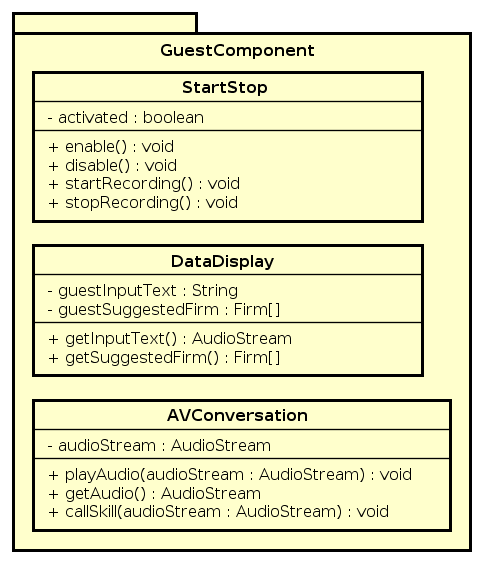
\includegraphics[scale=0.7]{Architettura/Front-End/GuestHome/GuestComponents.png}
		\caption{Schema del componente \texttt{Front-End :: GuestComponents}}
	\end{figure}
	\paragraph{Informazioni sul package}\begin{itemize}\item \textbf{Descrizione}: Package dedicato alla parte view e controller dell'interfaccia ospite\item \textbf{Padre}: GuestHome\item \textbf{Package contenuti}:
	\begin{itemize}\item Front-End :: GuestHome :: GuestComponents :: AVConversation: Componente che contiene al suo interno la sua view, il suo controller, ed i model di cui necessita
	\item Front-End :: GuestHome :: GuestComponents :: DataDisplay: Componente che contiene al suo interno la sua view, il suo controller, ed i model di cui necessita
	\item Front-End :: GuestHome :: GuestComponents :: StartStop: Componente che contiene al suo interno la sua view, il suo controller, ed i model di cui necessita
	\end{itemize}\paragraph{Classi}

	\newpage
	\subsubsection{\texttt{Front-End :: GuestHome :: GuestComponents :: StartStop}}

	\begin{figure}[!h]
		\centering
		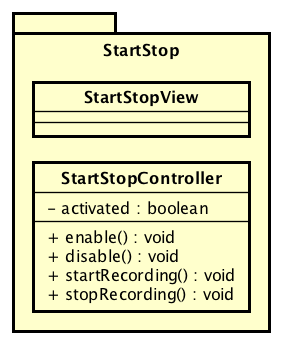
\includegraphics[scale=0.7]{Architettura/Front-End/GuestHome/Components/StartStop.png}
		\caption{Schema del componente \texttt{Front-End :: GuestComponents :: StartStop}}
	\end{figure}
	\begin{itemize}\item \textbf{Descrizione}: Classe contente tutti i metodi necessari a gestire l'attivazione e la disattivazione dell'AV
	\item \textbf{Utilizzo}: Verrà utilizzata per gestire l'Assistente Virtuale
	\item \textbf{Attributi}:
	\begin{itemize}
	\item \texttt{-activated: boolean}\

	 Attributo che indica se il sistema è in uno stato attivo o disattivo.
	\end{itemize}
	\item \textbf{Metodi}:
	\begin{itemize}
	\item \texttt{disable() : void}\

	 Funzione utilizzata per disattivare il sistema
	\end{itemize}\vspace{0.5em}
	\begin{itemize}
	\item \texttt{enable() : void}\

	 Funzione utilizzata per attivare il sistema
	\end{itemize}\vspace{0.5em}
	\begin{itemize}
	\item \texttt{startRecording() : void}\

	 Funzione utilizzata per cominciare una registrazione audio che verrà poi gestita da altre funzioni
	\end{itemize}\vspace{0.5em}
	\begin{itemize}
	\item \texttt{stopRecording() : void}\

	 Funzione utilizzata per terminare una registrazione audio che verrà poi gestita da altre funzioni

	\end{itemize}\vspace{0.5em}
	\item \textbf{Relazioni con altre classi}:
	\begin{itemize}
	\item \texttt{Front-End :: GuestHome :: GuestServices :: InteractionService}: Contiene i servizi con cui si interfacciano i component di Angular per il client dell'ospite.
	\end{itemize}
	\end{itemize}\end{itemize}

	\newpage
	\subsubsection{ \texttt{Front-End :: GuestHome :: GuestComponents :: AVConversation}}
	\begin{figure}[!h]
		\centering
		\includegraphics[scale=0.7]{Architettura/Front-End/GuestHome/Components/Conversation.png}
		\caption{Schema del componente \texttt{Front-End :: GuestComponents :: AVConversation}}
	\end{figure}
	\paragraph{Informazioni sul package}\begin{itemize}\item \textbf{Descrizione}: Componente che contiene al suo interno la sua view, il suo controller, ed i model di cui necessita\item \textbf{Padre}: GuestComponents\paragraph{Classi}
	\subparagraph{\texttt{Front-End :: GuestHome :: GuestComponents :: AVConversation :: AVConversationController}}
	\begin{itemize}\item \textbf{Descrizione}: Classe che si occupa di effettuare la conversazione tra ospite e AV
	\item \textbf{Utilizzo}: Sarà utilizzata per permettere la conversazione tra ospite e Assistente Virtuale
	\item \textbf{Attributi}:
	\begin{itemize}
	\item \texttt{-AudioStream: AudioStream}\

	 Attributo per indicare lo stream audio che sarà riprodotto dall'AV.
	\end{itemize}
	\item \textbf{Metodi}:
	\begin{itemize}
	\item \texttt{callSkill(audioStream) : void}\

	 Funzione utilizzata per chiamare una skill inviando una traccia audio

	\item \textbf{Argomenti}:
	\begin{itemize}
	\item \texttt{audioStream : AudioStream}\

	 Parametro che indica la traccia audio di tipo AudioStream da inviare alla skill chiamata.
	\end{itemize}
	\end{itemize}\vspace{0.5em}
	\begin{itemize}
	\item \texttt{getAudio() : AudioStream}\

	 Funzione utilizzata per ottenere una traccia audio di tipo AudioStream da gestire
	\end{itemize}\vspace{0.5em}
	\begin{itemize}
	\item \texttt{playAudio(audioStream) : void}\

	 Funzione utilizzata per riprodurre una traccia audio di tipo AudioStream

	\item \textbf{Argomenti}:
	\begin{itemize}
	\item \texttt{audioStream : AudioStream}\

	 Parametro che indica la traccia audio da gestire.
	\end{itemize}
	\end{itemize}\vspace{0.5em}
	\end{itemize}\subparagraph{\texttt{Front-End :: GuestHome :: GuestComponents :: AVConversation :: AVConversationView}}
	\begin{itemize}\item \textbf{Descrizione}: Classe utilizzata per visualizzare la conversazione tra ospite e AV
	\item \textbf{Utilizzo}: View di AVConversation
	\end{itemize}\end{itemize}

	\newpage
	\subsubsection{ \texttt{Front-End :: GuestHome :: GuestComponents :: DataDisplay}}
	\begin{figure}[!h]
		\centering
		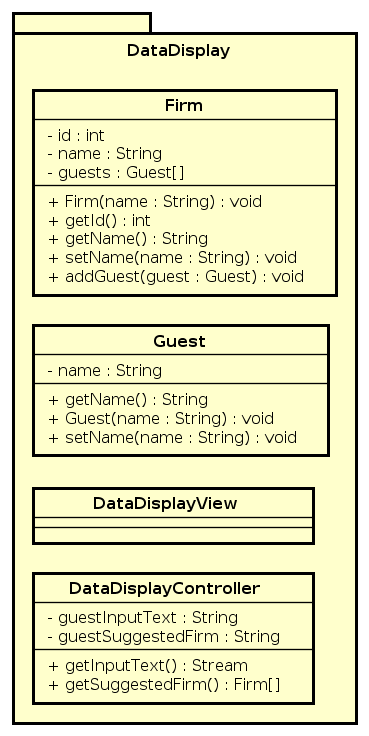
\includegraphics[scale=0.7]{Architettura/Front-End/GuestHome/Components/DataDisplay.png}
		\caption{Schema del componente \texttt{Front-End :: GuestComponents :: DataDisplay}}
	\end{figure}
	\paragraph{Informazioni sul package}\begin{itemize}\item \textbf{Descrizione}: Componente che contiene al suo interno la sua view, il suo controller, ed i model di cui necessita\item \textbf{Padre}: GuestComponents\paragraph{Classi}
	\subparagraph{\texttt{Front-End :: GuestHome :: GuestComponents :: DataDisplay :: DataDisplayController}}
	\begin{itemize}\item \textbf{Descrizione}: Classe contenente tutti i metodi necessari a mostrare a schermo informazioni utili all'utente o ospite
	\item \textbf{Utilizzo}: Verrà utilizzata per fornire informazioni all'utente o ospite
	\item \textbf{Attributi}:
	\begin{itemize}
	\item \texttt{-guestInputText: string}\

	 Attributo che indica il testo che l'utente dovrebbe aver detto, quindi che Alexa ha capito.
	\end{itemize}
	\begin{itemize}
	\item \texttt{-guestSuggestedFirm: Firm[]}\

	 Attributo che indica una lista di aziende che vengono suggerite all'utente che interagisce con l'AV.
	\end{itemize}
	\item \textbf{Metodi}:
	\begin{itemize}
	\item \texttt{getInputText() : AudioStream}\

	 Funzione utilizzata per ottenere e mostrare a video il testo che Alexa ha compreso dall'AudioStream ricevuto
	\end{itemize}\vspace{0.5em}
	\begin{itemize}
	\item \texttt{getSuggestedFirm() : Firm[]}\

	 Funzione che riceve e mostra a video le aziende da suggerire all'utente
	\end{itemize}\vspace{0.5em}
	\end{itemize}\subparagraph{\texttt{Front-End :: GuestHome :: GuestComponents :: DataDisplay :: DataDisplayView}}
	\begin{itemize}\item \textbf{Descrizione}: Classe contenente tutti i metodi necessari a mostrare a schermo informazioni utili all'utente o ospite
	\item \textbf{Utilizzo}: View di DataDisplay
	\end{itemize}\end{itemize}
	\subsubsection{ \texttt{Front-End :: GuestHome :: GuestComponents :: StartStop}}\paragraph{Informazioni sul package}\begin{itemize}\item \textbf{Descrizione}: Componente che contiene al suo interno la sua view, il suo controller, ed i model di cui necessita\item \textbf{Padre}: GuestComponents\end{itemize}

	\newpage
	\subsubsection{ \texttt{Front-End :: GuestHome :: GuestServices}}
	\begin{figure}[!h]
		\centering
		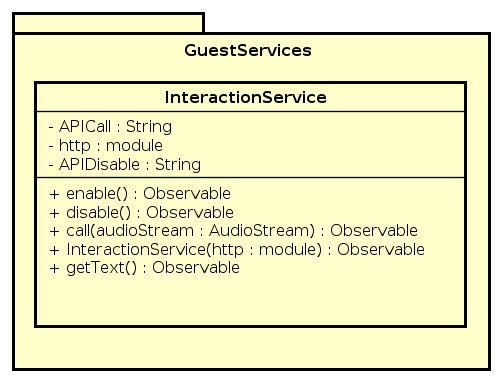
\includegraphics[scale=0.7]{Architettura/Front-End/GuestHome/GuestServices.png}
		\caption{Schema del componente \texttt{Back-End :: GuestServices}}
	\end{figure}
	\paragraph{Informazioni sul package}\begin{itemize}\item \textbf{Descrizione}: Package dedicato ai servizi disponibili agli ospiti \item \textbf{Padre}: GuestHome\paragraph{Classi}
	\subparagraph{\texttt{Front-End :: GuestHome :: GuestServices :: InteractionService}}
	\begin{itemize}\item \textbf{Descrizione}: Contiene i servizi con cui si interfacciano i component di Angular per il client dell'ospite.
	\item \textbf{Utilizzo}: Servizi per i component dell'ospite.
	\item \textbf{Attributi}:
	\begin{itemize}
	\item \texttt{-APICall: string}\

	 Percorso per l'API call.
	\end{itemize}
	\begin{itemize}
	\item \texttt{-APIDisable: string}\

	 Perorso per l'API disable.
	\end{itemize}
	\begin{itemize}
	\item \texttt{-http: Module}\

	 Modulo per la chiamata http.
	\end{itemize}
	\item \textbf{Metodi}:
	\begin{itemize}
	\item \texttt{call(audiostream) : Observable}\

	 Chiama la Lambda Skill utilizzando il percorso contenuto nell'attributo di APICall, usando lo stream audio registrato.

	\item \textbf{Argomenti}:
	\begin{itemize}
	\item \texttt{audiostream : AudioStream}\

	 Parametro che contiene lo stream audio.
	\end{itemize}
	\end{itemize}\vspace{0.5em}
	\begin{itemize}
	\item \texttt{disable() : Observable}\

	 Chiude una conversazione aperta.
	\end{itemize}\vspace{0.5em}
	\begin{itemize}
	\item \texttt{enable() : Observable}\

	 Apre una nuova conversazione.
	\end{itemize}\vspace{0.5em}
	\begin{itemize}
	\item \texttt{getText() : Observable}\

	 Ritorna il testo della chiamata sotto forma di Observable.
	\end{itemize}\vspace{0.5em}
	\begin{itemize}
	\item \texttt{InteractionService(http) : Observable}\

	 Costruttore, ritorna un tipo Observable per le specifiche di Angular2.

	\item \textbf{Argomenti}:
	\begin{itemize}
	\item \texttt{http : Module}\

	 Modulo per la chiamata http passato in input per la costruzione del service.
	\end{itemize}
	\end{itemize}\vspace{0.5em}
	\end{itemize}\end{itemize}

\subsection{ \texttt{Models}}
\begin{figure}[!h]
	\centering
	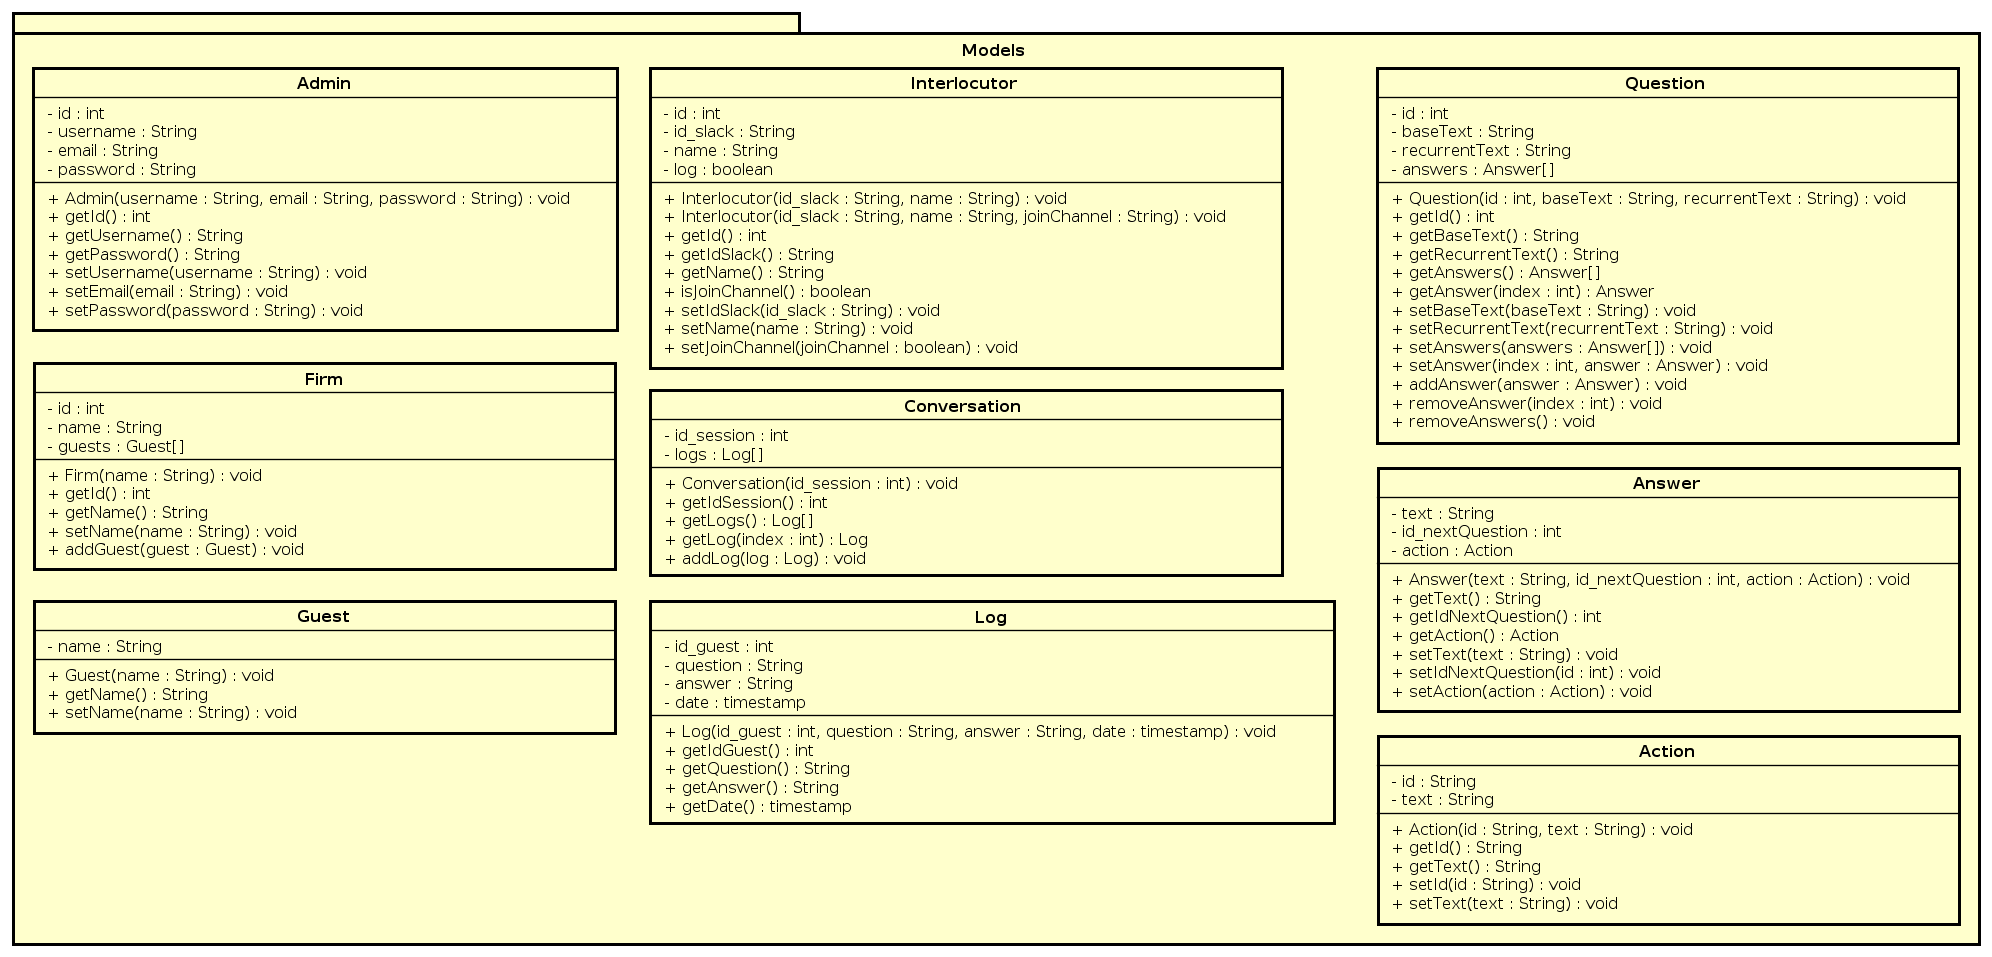
\includegraphics[width=\textwidth]{Architettura/Models.png}
	\caption{Schema del componente \texttt{Models}}
\end{figure}
\paragraph{Informazioni sul package}\begin{itemize}\item \textbf{Descrizione}: Package che contiene tutti i models\paragraph{Classi}

	\newpage
	\subsubsection{\texttt{Models :: Action}}
	\begin{figure}[!h]
		\centering
		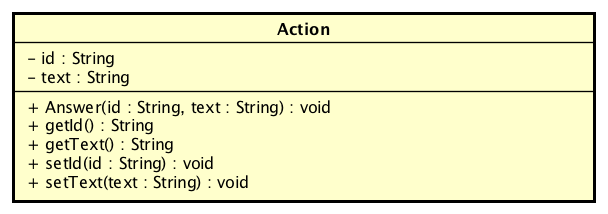
\includegraphics[scale=0.7]{Architettura/Models/Action.png}
		\caption{Schema del componente \texttt{Models :: Action}}
	\end{figure}

	\begin{itemize}\item \textbf{Descrizione}: Rappresenta un'azione predefinita e ne contiene tutte le informazioni necessarie alla presentazione del suo contenuto
	\item \textbf{Utilizzo}: Viene utilizzata per memorizzare i dati di un'azione predefinita
	\item \textbf{Attributi}:
	\begin{itemize}
	\item \texttt{id: string}\

	 Attributo che rappresenta l'id di un'azione predefinita.
	\end{itemize}
	\begin{itemize}
	\item \texttt{text: string}\

	 Attributo che rappresenta il testo di un'azione predefinita.
	\end{itemize}
	\item \textbf{Metodi}:
	\begin{itemize}
	\item \texttt{Action(id, text) : void}\

	 Costruttore

	\item \textbf{Argomenti}:
	\begin{itemize}
	\item \texttt{id : string}\

	 ID dell'Action.
	\item \texttt{text : string}\

	 Testo descrittivo dell'Action.
	\end{itemize}
	\end{itemize}\vspace{0.5em}
	\begin{itemize}
	\item \texttt{getId() : string}\

	 Getter dell'ID
	\end{itemize}\vspace{0.5em}
	\begin{itemize}
	\item \texttt{setId() : void}\

	 Setter dell'ID
	\end{itemize}\vspace{0.5em}
	\begin{itemize}
	\item \texttt{setText() : void}\

	 Setter del testo descrittivo
	\end{itemize}\vspace{0.5em}
	\begin{itemize}
	\item \texttt{getText() : string}\

	 Getter del testo descrittivo
	\end{itemize}\vspace{0.5em}
	\item \textbf{Relazioni con altre classi}:
	\begin{itemize}
	\item \texttt{Front-End :: AdministrationView :: AdminComponents :: ManageQuestions :: ManageQuestionsController}: Componente per le domande e interazioni.
	\end{itemize}

	\end{itemize}

	\newpage
	\subsubsection{\texttt{Models :: Admin}}
	\begin{figure}[!h]
		\centering
		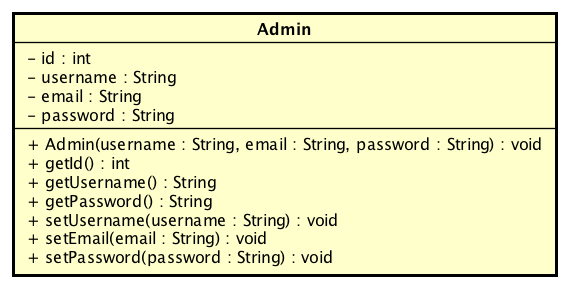
\includegraphics[scale=0.7]{Architettura/Models/Admin.png}
		\caption{Schema del componente \texttt{Models :: Admin}}
	\end{figure}
	\begin{itemize}\item \textbf{Descrizione}: Rappresenta un amministratore e ne contiene tutte le informazioni necessarie alla presentazione del suo contenuto
	\item \textbf{Utilizzo}: Viene utilizzata per memorizzare i dati di un amministratore
	\item \textbf{Attributi}:
	\begin{itemize}
	\item \texttt{id: int}\

	 Attributo che rappresenta l'id di un amministratore.
	\end{itemize}
	\begin{itemize}
	\item \texttt{password: string}\

	 Attributo che rappresenta la email di un amministratore.
	\end{itemize}
	\begin{itemize}
	\item \texttt{username: string}\

	 Attributo che rappresenta lo username di un amministratore.
	\end{itemize}
	\item \textbf{Metodi}:
	\begin{itemize}
	\item \texttt{Admin(password, username) : void}\

	 Costruttore del modello Admin

	\item \textbf{Argomenti}:
	\begin{itemize}
	\item \texttt{password : string}\

	 Parametro che indica la password dell'amministratore.
	\item \texttt{username : string}\

	 Parametro che indica lo username dell'amministratore.
	\end{itemize}
	\end{itemize}\vspace{0.5em}
	\begin{itemize}
	\item \texttt{getId() : int}\

	 Funzione che permette di ottenere l'id dell'amministratore
	\end{itemize}\vspace{0.5em}
	\begin{itemize}
	\item \texttt{getPassword() : string}\

	 Funzione che permette di ottenere la password di un amministratore
	\end{itemize}\vspace{0.5em}
	\begin{itemize}
	\item \texttt{getUsername() : string}\

	 Funzione che permette di ottenere lo username di un amministratore
	\end{itemize}\vspace{0.5em}
	\begin{itemize}
	\item \texttt{setEmail(email) : void}\

	 Funzione che permette di modificare la email di un amministratore

	\item \textbf{Argomenti}:
	\begin{itemize}
	\item \texttt{email : string}\

	 Parametro che indica la nuova email di un amministratore.
	\end{itemize}
	\end{itemize}\vspace{0.5em}
	\begin{itemize}
	\item \texttt{setPassword(password) : void}\

	 Funzione che permette di modificare la password di un amministratore

	\item \textbf{Argomenti}:
	\begin{itemize}
	\item \texttt{password : string}\

	 Parametro che indica la nuova password di un amministratore.
	\end{itemize}
	\end{itemize}\vspace{0.5em}
	\begin{itemize}
	\item \texttt{setUsername(username) : void}\

	 Funzione che permette di modificare lo username di un amministratore

	\item \textbf{Argomenti}:
	\begin{itemize}
	\item \texttt{username : string}\

	 Parametro che indica il nuovo username dell'amministratore.
	\end{itemize}
	\end{itemize}\vspace{0.5em}
	\item \textbf{Relazioni con altre classi}:
	\begin{itemize}
	\item \texttt{Front-End :: AdministrationView :: AdminComponents :: ManageAdministrators :: ManageAdministratorsController}: Controller che gestisce la view di ManageAdministrators permettendo ad un SuperAdmin di gestire le informazioni degli altri amministratori;
	\item \texttt{Front-End :: AdministrationView :: AdminComponents :: ManageProfile :: ManageProfileController}: Controller che gestisce la view di ManageProfileView permettendo ad un amministratore di gestire il proprio profilo nell'area amministrativa.
	\end{itemize}

	\end{itemize}

	\newpage
	\subsubsection{\texttt{Models :: Answer}}
	\begin{figure}[!h]
		\centering
		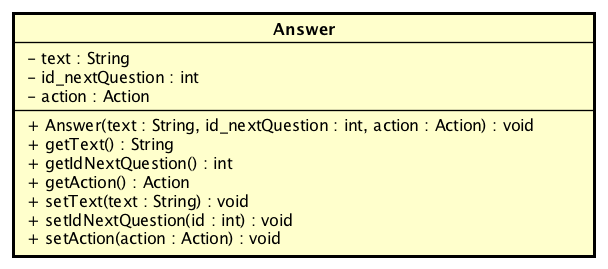
\includegraphics[scale=0.7]{Architettura/Models/Answer.png}
		\caption{Schema del componente \texttt{Models :: Answer}}
	\end{figure}
	\begin{itemize}\item \textbf{Descrizione}: Rappresenta una risposta e ne contiene tutte le informazioni necessarie alla presentazione del suo contenuto
	\item \textbf{Utilizzo}: Viene utilizzata per memorizzare i dati di una risposta
	\item \textbf{Attributi}:
	\begin{itemize}
	\item \texttt{action: Action}\

	 Attributo che rappresenta l'azione predefinita da eseguire legata ad una risposta.
	\end{itemize}
	\begin{itemize}
	\item \texttt{id\_nextQuestion: int}\

	 Attributo che rappresenta l'id della prossima domanda legata ad una risposta.
	\end{itemize}
	\begin{itemize}
	\item \texttt{text: string}\

	 Attributo che rappresenta il testo di una risposta.
	\end{itemize}
	\item \textbf{Metodi}:
	\begin{itemize}
	\item \texttt{Answer(action, text) : void}\

	 Costruttore

	\item \textbf{Argomenti}:
	\begin{itemize}
	\item \texttt{action : Action}\

	 Azione da eseguire.
	\item \texttt{text : string}\

	 Testo della risposta.
	\end{itemize}
	\end{itemize}\vspace{0.5em}
	\begin{itemize}
	\item \texttt{getAction() : Action}\

	 Getter dell'azione da eseguire
	\end{itemize}\vspace{0.5em}
	\begin{itemize}
	\item \texttt{getIdNextQuestion() : int}\

	 Getter dell'ID della prossima domanda da porre
	\end{itemize}\vspace{0.5em}
	\begin{itemize}
	\item \texttt{getText() : string}\

	 Getter del testo
	\end{itemize}\vspace{0.5em}
	\begin{itemize}
	\item \texttt{setAction() : void}\

	 Setter dell'Action
	\end{itemize}\vspace{0.5em}
	\begin{itemize}
	\item \texttt{setIdNextQuestion(id) : void}\

	 Setter dell'ID della prossima domanda da porre

	\item \textbf{Argomenti}:
	\begin{itemize}
	\item \texttt{id : int}\

	 ID della prossima domanda.
	\end{itemize}
	\end{itemize}\vspace{0.5em}
	\begin{itemize}
	\item \texttt{setText() : void}\

	 Setter del testo della risposta
	\end{itemize}\vspace{0.5em}
	\item \textbf{Relazioni con altre classi}:
	\begin{itemize}
	\item \texttt{Front-End :: AdministrationView :: AdminComponents :: ManageQuestions :: ManageQuestionsController}: Componente per le domande e interazioni.
	\end{itemize}
	\end{itemize}

	\newpage
	\subsubsection{\texttt{Models :: Conversation}}
	\begin{figure}[!h]
		\centering
		\includegraphics[scale=0.7]{Architettura/Models/Conversation.png}
		\caption{Schema del componente \texttt{Models :: Conversation}}
	\end{figure}
	\begin{itemize}\item \textbf{Descrizione}: Rappresenta una conversazione e ne contiene tutte le informazioni necessarie alla presentazione del suo contenuto
	\item \textbf{Utilizzo}: Viene utilizzata per memorizzare i dati di una conversazione
	\item \textbf{Attributi}:
	\begin{itemize}
	\item \texttt{id\_session: int}\

	 Attributo che rappresenta la session\_id di un conversazione.
	\end{itemize}
	\begin{itemize}
	\item \texttt{logs: Log[]}\

	 Attributo che rappresenta l'insieme dei log di una conversazione
	.
	\end{itemize}
	\item \textbf{Metodi}:
	\begin{itemize}
	\item \texttt{addLog(log) : void}\

	 Funzione che permette di aggiungere un log alla conversazione

	\item \textbf{Argomenti}:
	\begin{itemize}
	\item \texttt{log : Log}\

	 Parametro che indica il nuovo log da aggiungere alla conversazione.
	\end{itemize}
	\end{itemize}\vspace{0.5em}
	\begin{itemize}
	\item \texttt{Conversation(id\_session) : void}\

	 Costruttore del model Conversation

	\item \textbf{Argomenti}:
	\begin{itemize}
	\item \texttt{id\_session : int}\

	 Parametro che indica l'id\_session della sessione di Alexa.
	\end{itemize}
	\end{itemize}\vspace{0.5em}
	\begin{itemize}
	\item \texttt{getIdSession() : int}\

	 Funzione che permette di ottenere l'id\_session di una conversazione
	\end{itemize}\vspace{0.5em}
	\begin{itemize}
	\item \texttt{getLog() : Log}\

	 Funzione che permette di ottenere uno specifico log di una conversazione
	\end{itemize}\vspace{0.5em}
	\begin{itemize}
	\item \texttt{getLogs() : Log[]}\

	 Funzione che permette di ottenere l'insieme dei log di una conversazione
	\end{itemize}\vspace{0.5em}
	\item \textbf{Relazioni con altre classi}:
	\begin{itemize}
	\item \texttt{Front-End :: AdministrationView :: AdminComponents :: ManageFirms :: ManageFirmsController}: Componente per la scelta degli oggetti di tipo Firm.
	\end{itemize}

	\end{itemize}

	\newpage
	\subsubsection{\texttt{Models :: Firm}}
	\begin{figure}[!h]
		\centering
		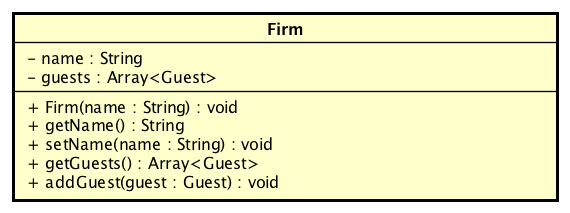
\includegraphics[scale=0.7]{Architettura/Models/Firm.png}
		\caption{Schema del componente \texttt{Models :: Firm}}
	\end{figure}
	\begin{itemize}\item \textbf{Descrizione}: Rappresenta un'azienda e ne contiene tutte le informazioni necessarie alla presentazione del suo contenuto
	\item \textbf{Utilizzo}: Viene utilizzata per memorizzare i dati di un'azienda
	\item \textbf{Attributi}:
	\begin{itemize}
	\item \texttt{guests: Guest[]}\

	 Attributo che rappresenta gli ospiti registrati di un'azienda.
	\end{itemize}
	\begin{itemize}
	\item \texttt{id: int}\

	 Attributo che rappresenta l'id di un'azienda.
	\end{itemize}
	\begin{itemize}
	\item \texttt{name: string}\

	 Attributo che rappresenta il nome di un'azienda.
	\end{itemize}
	\item \textbf{Metodi}:
	\begin{itemize}
	\item \texttt{addGuest(guest) : void}\

	 Funzione che permette di aggiungere un nuovo ospiti ad un'azienda

	\item \textbf{Argomenti}:
	\begin{itemize}
	\item \texttt{guest : Guest}\

	 Parametro che indica l'ospite da aggiungere all'azienda.
	\end{itemize}
	\end{itemize}\vspace{0.5em}
	\begin{itemize}
	\item \texttt{Firm(name) : void}\

	 Costruttore del model azienda

	\item \textbf{Argomenti}:
	\begin{itemize}
	\item \texttt{name : string}\

	 Parametro che indica il nome di un'azienda.
	\end{itemize}
	\end{itemize}\vspace{0.5em}
	\begin{itemize}
	\item \texttt{getId() : int}\

	 Funzione che permette di ottenere l'id di un'azienda
	\end{itemize}\vspace{0.5em}
	\begin{itemize}
	\item \texttt{getName() : string}\

	 Funzione che permette di ottenere il nome di un'azienda
	\end{itemize}\vspace{0.5em}
	\begin{itemize}
	\item \texttt{setName(name) : void}\

	 Funzione che permette di modificare il nome di un'azienda

	\item \textbf{Argomenti}:
	\begin{itemize}
	\item \texttt{name : string}\

	 Parametro che indica il nuovo nome dell'azienda.
	\end{itemize}
	\end{itemize}\vspace{0.5em}
	\item \textbf{Relazioni con altre classi}:
	\begin{itemize}
	\item \texttt{Front-End :: AdministrationView :: AdminComponents :: ManageFirms :: ManageFirmsController}: Componente per la scelta degli oggetti di tipo Firm.
	\end{itemize}

	\end{itemize}

	\newpage
	\subsubsection{\texttt{Models :: Guest}}
	\begin{figure}[!h]
		\centering
		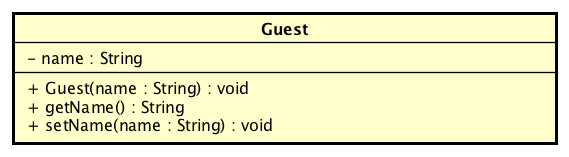
\includegraphics[scale=0.7]{Architettura/Models/Guest.png}
		\caption{Schema del componente \texttt{Models :: Guest}}
	\end{figure}
	\begin{itemize}\item \textbf{Descrizione}: Rappresenta un ospite e ne contiene tutte le informazioni necessarie alla presentazione del suo contenuto
	\item \textbf{Utilizzo}: Viene utilizzata per memorizzare i dati di un ospite
	\item \textbf{Attributi}:
	\begin{itemize}
	\item \texttt{name: string}\

	 Attributo che rappresenta il nome di un ospite
	.
	\end{itemize}
	\item \textbf{Metodi}:
	\begin{itemize}
	\item \texttt{getName() : string}\

	 Funzione che permette di ottenere il nome di un guest
	\end{itemize}\vspace{0.5em}
	\begin{itemize}
	\item \texttt{Guest() : void}\

	 Costruttore del modello Guest
	\end{itemize}\vspace{0.5em}
	\begin{itemize}
	\item \texttt{setName() : void}\

	 Funzione che permette di modificare il nome di un ospite
	\end{itemize}\vspace{0.5em}
	\item \textbf{Relazioni con altre classi}:
	\begin{itemize}
	\item \texttt{Front-End :: AdministrationView :: AdminComponents :: ManageFirms :: ManageFirmsController}: Componente per la scelta degli oggetti di tipo Firm.
	\end{itemize}
	\end{itemize}

	\newpage
	\subsubsection{\texttt{Models :: Interlocutor}}
	\begin{figure}[!h]
		\centering
		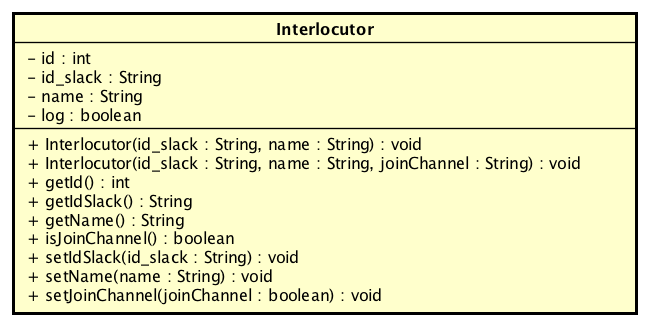
\includegraphics[scale=0.7]{Architettura/Models/Interlocutor.png}
		\caption{Schema del componente \texttt{Models :: Interlocutor}}
	\end{figure}
	\begin{itemize}\item \textbf{Descrizione}: Rappresenta un interlocutore e ne contiene tutte le informazioni necessarie alla presentazione del suo contenuto
	\item \textbf{Utilizzo}: Viene utilizzata per memorizzare i dati di un interlocutore
	\item \textbf{Attributi}:
	\begin{itemize}
	\item \texttt{id: int}\

	 Attributo che rappresenta l'id di un interlocutore
	.
	\end{itemize}
	\begin{itemize}
	\item \texttt{id\_slack: string}\

	 Attributo che rappresenta l'id di Slack di un interlocutore
	.
	\end{itemize}
	\begin{itemize}
	\item \texttt{joined: string}\

	 Attributo che indica se un interlocutore è associato o meno alla lista di default \#azienda.
	\end{itemize}
	\begin{itemize}
	\item \texttt{name: string}\

	 Attributo che rappresenta il nome di un interlocutore
	.
	\end{itemize}
	\item \textbf{Metodi}:
	\begin{itemize}
	\item \texttt{getId() : int}\

	 Funzione che permette di ottenere l'id di un interlocutore
	\end{itemize}\vspace{0.5em}
	\begin{itemize}
	\item \texttt{getIdSlack() : string}\

	 Funzione che permette di ottenere l'id\_slack di un interlocutore
	\end{itemize}\vspace{0.5em}
	\begin{itemize}
	\item \texttt{getName() : string}\

	 Funzione che permette di ottenere il nome di un interlocutore
	\end{itemize}\vspace{0.5em}
	\begin{itemize}
	\item \texttt{Interlocutor(id\_slack) : void}\

	 Costruttore del modello Interlocutor

	\item \textbf{Argomenti}:
	\begin{itemize}
	\item \texttt{id\_slack : string}\

	 Parametro che indica l'id Slack dell'interlocutore.
	\end{itemize}
	\end{itemize}\vspace{0.5em}
	\begin{itemize}
	\item \texttt{Interlocutor(id\_slack) : void}\

	 Costruttore del modello Interlocutor

	\item \textbf{Argomenti}:
	\begin{itemize}
	\item \texttt{id\_slack : string}\

	 Parametro che indica l'id Slack dell'interlocutore.
	\end{itemize}
	\end{itemize}\vspace{0.5em}
	\begin{itemize}
	\item \texttt{setIdSlack(id\_slack) : void}\

	 Funzione che permette di modificare l'id\_slack di un interlocutore

	\item \textbf{Argomenti}:
	\begin{itemize}
	\item \texttt{id\_slack : string}\

	 Parametro che indica il nuovo id\_slack di un interlocutore.
	\end{itemize}
	\end{itemize}\vspace{0.5em}
	\begin{itemize}
	\item \texttt{setJoinChannel(joinChannel) : void}\

	 Funzione che permette di modificare l'associazione di un interlocutore alla lista di defaut \#azienda

	\item \textbf{Argomenti}:
	\begin{itemize}
	\item \texttt{joinChannel : boolean}\

	 Parametro che indica l'assocazione o meno di un interlocutore alla lista di default \#azienda.
	\end{itemize}
	\end{itemize}\vspace{0.5em}
	\begin{itemize}
	\item \texttt{setName() : void}\

	 Funzione che permette di modificare il nome di un interlocutore
	\end{itemize}\vspace{0.5em}
	\begin{itemize}
	\item \texttt{isJoinChannel() : boolean}\

	 Funzione che permette di sapere se un interlocutore è associato alla lista di default \#azienda
	\end{itemize}\vspace{0.5em}
	\item \textbf{Relazioni con altre classi}:
	\begin{itemize}
	\item \texttt{Front-End :: AdministrationView :: AdminComponents :: ManageSlack :: ManageSlackController}: Componente per la gestione dei canali Slack.
	\end{itemize}
	\end{itemize}

	\newpage
	\subsubsection{\texttt{Models :: Log}}
	\begin{figure}[!h]
		\centering
		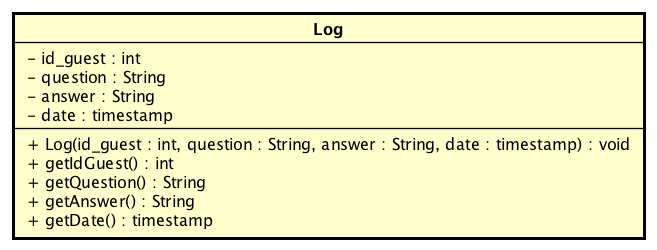
\includegraphics[scale=0.7]{Architettura/Models/Log.png}
		\caption{Schema del componente \texttt{Models :: Log}}
	\end{figure}
	\begin{itemize}\item \textbf{Descrizione}: Rappresenta un log e ne contiene tutte le informazioni necessarie alla presentazione del suo contenuto
	\item \textbf{Utilizzo}: Viene utilizzata per memorizzare i dati di un log
	\item \textbf{Attributi}:
	\begin{itemize}
	\item \texttt{answer: string}\

	 Attributo che rappresenta la risposta legata ad un log
	.
	\end{itemize}
	\begin{itemize}
	\item \texttt{date: string}\

	 Attributo che rappresenta la data legata ad un log.
	\end{itemize}
	\begin{itemize}
	\item \texttt{id\_guest: int}\

	 Attributo che rappresenta l'id dell'ospite in un log.
	\end{itemize}
	\begin{itemize}
	\item \texttt{question: string}\

	 Attributo che rappresenta la domanda legata ad un log.
	\end{itemize}
	\item \textbf{Metodi}:
	\begin{itemize}
	\item \texttt{getAnswer() : string}\

	 Funzione che permette di ottenere il testo della risposta legato ad un log
	\end{itemize}\vspace{0.5em}
	\begin{itemize}
	\item \texttt{getDate() : string}\

	 Funzione che permette di ottenere la data legata ad un log
	\end{itemize}\vspace{0.5em}
	\begin{itemize}
	\item \texttt{getDate() : string}\

	 Getter del timestamp del log
	\end{itemize}\vspace{0.5em}
	\begin{itemize}
	\item \texttt{getIdGuest() : int}\

	 Funzione che permette di ottenere l'id\_guest legato ad un log
	\end{itemize}\vspace{0.5em}
	\begin{itemize}
	\item \texttt{getQuestion() : string}\

	 Funzione che permette di ottenere il testo della domanda legato ad un log
	\end{itemize}\vspace{0.5em}
	\begin{itemize}
	\item \texttt{Log(date, id\_guest, question) : void}\

	 Costruttore del modello Log

	\item \textbf{Argomenti}:
	\begin{itemize}
	\item \texttt{date : string}\

	 Parametro che indica la data legata al log.
	\item \texttt{id\_guest : int}\

	 Parametro che indica l'id\_guest legato al Log.
	\item \texttt{question : string}\

	 Parametro che indica il testo della domanda legata al log.
	\end{itemize}
	\end{itemize}\vspace{0.5em}
	\item \textbf{Relazioni con altre classi}:
	\begin{itemize}
	\item \texttt{Front-End :: AdministrationView :: AdminComponents :: ManageFirms :: ManageFirmsController}: Componente per la scelta degli oggetti di tipo Firm.
	\end{itemize}
	\end{itemize}

	\newpage
	\subsubsection{\texttt{Models :: Question}}
	\begin{figure}[!h]
		\centering
		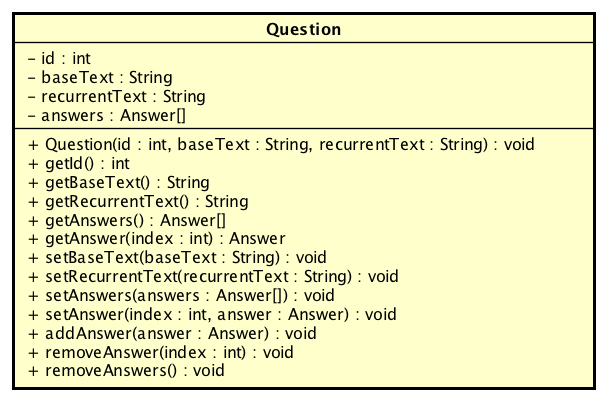
\includegraphics[scale=0.7]{Architettura/Models/Question.png}
		\caption{Schema del componente \texttt{Models :: Question}}
	\end{figure}
	\begin{itemize}\item \textbf{Descrizione}: Rappresenta una domanda e ne contiene tutte le informazioni necessarie alla presentazione del suo contenuto
	\item \textbf{Utilizzo}: Viene utilizzata per memorizzare i dati di una domanda
	\item \textbf{Attributi}:
	\begin{itemize}
	\item \texttt{answers: Answer[]}\

	 Attributo che rappresenta l'insieme delle risposte allegate ad una domanda.
	\end{itemize}
	\begin{itemize}
	\item \texttt{baseText: string}\

	 Attributo che rappresenta il testo base di una domanda.
	\end{itemize}
	\begin{itemize}
	\item \texttt{id: int}\

	 Attributo che rappresenta l'id di una domanda.
	\end{itemize}
	\begin{itemize}
	\item \texttt{recurrentText: string}\

	 Attributo che rappresenta il testo ricorrente di una domanda.
	\end{itemize}
	\item \textbf{Metodi}:
	\begin{itemize}
	\item \texttt{addAnswer(answer) : void}\

	 Aggiunge una risposta

	\item \textbf{Argomenti}:
	\begin{itemize}
	\item \texttt{answer : Answer}\

	 Risposta.
	\end{itemize}
	\end{itemize}\vspace{0.5em}
	\begin{itemize}
	\item \texttt{getAnswer(index) : Action}\

	 Ricerca di una riposta tramite indice

	\item \textbf{Argomenti}:
	\begin{itemize}
	\item \texttt{index : int}\

	 Indice della risposta.
	\end{itemize}
	\end{itemize}\vspace{0.5em}
	\begin{itemize}
	\item \texttt{getAnswers() : Answer[]}\

	 Getter delle risposte
	\end{itemize}\vspace{0.5em}
	\begin{itemize}
	\item \texttt{getBaseText() : string}\

	 Getter del testo base
	\end{itemize}\vspace{0.5em}
	\begin{itemize}
	\item \texttt{getId() : int}\

	 Getter dell'ID della domanda
	\end{itemize}\vspace{0.5em}
	\begin{itemize}
	\item \texttt{getRecurrentText() : string}\

	 Getter del testo ricorrente
	\end{itemize}\vspace{0.5em}
	\begin{itemize}
	\item \texttt{Question(id) : void}\

	 Costruttore

	\item \textbf{Argomenti}:
	\begin{itemize}
	\item \texttt{id : int}\

	 Id della domanda.
	\end{itemize}
	\end{itemize}\vspace{0.5em}
	\begin{itemize}
	\item \texttt{removeAnswer(index) : void}\

	 Rimuove una domanda

	\item \textbf{Argomenti}:
	\begin{itemize}
	\item \texttt{index : int}\

	 indice della domanda da rimuovere.
	\end{itemize}
	\end{itemize}\vspace{0.5em}
	\begin{itemize}
	\item \texttt{removeAnswers() : void}\

	 Rimuove tutte le risposte
	\end{itemize}\vspace{0.5em}
	\begin{itemize}
	\item \texttt{setAnswer() : void}\

	 Setter di una risposta
	\end{itemize}\vspace{0.5em}
	\begin{itemize}
	\item \texttt{setAnswers() : void}\

	 Setter delle risposte
	\end{itemize}\vspace{0.5em}
	\begin{itemize}
	\item \texttt{setBaseText() : void}\

	 Setter del testo base
	\end{itemize}\vspace{0.5em}
	\begin{itemize}
	\item \texttt{setRecurrentText(recurrentText) : void}\

	 Setter del testo ricorrente

	\item \textbf{Argomenti}:
	\begin{itemize}
	\item \texttt{recurrentText : string}\

	 Testo ricorrente.
	\end{itemize}
	\end{itemize}\vspace{0.5em}
	\item \textbf{Relazioni con altre classi}:
	\begin{itemize}
	\item \texttt{Front-End :: AdministrationView :: AdminComponents :: ManageQuestions :: ManageQuestionsController}: Componente per le domande e interazioni.
	\end{itemize}
	\end{itemize}\end{itemize}


\subsection{ \texttt{Angular 2}}\paragraph{Informazioni sul package}\begin{itemize}\item \textbf{Descrizione}: Package che si riferisce al componente esterno Angular 2 che si utilizza nell'architettura\end{itemize}

\subsection{ \texttt{APIGateway}}\paragraph{Informazioni sul package}\begin{itemize}\item \textbf{Descrizione}: Package dedicato all'interfaccia REST\end{itemize}



\subsection{ \texttt{Back-End}}
\begin{figure}[!h]
	\centering
	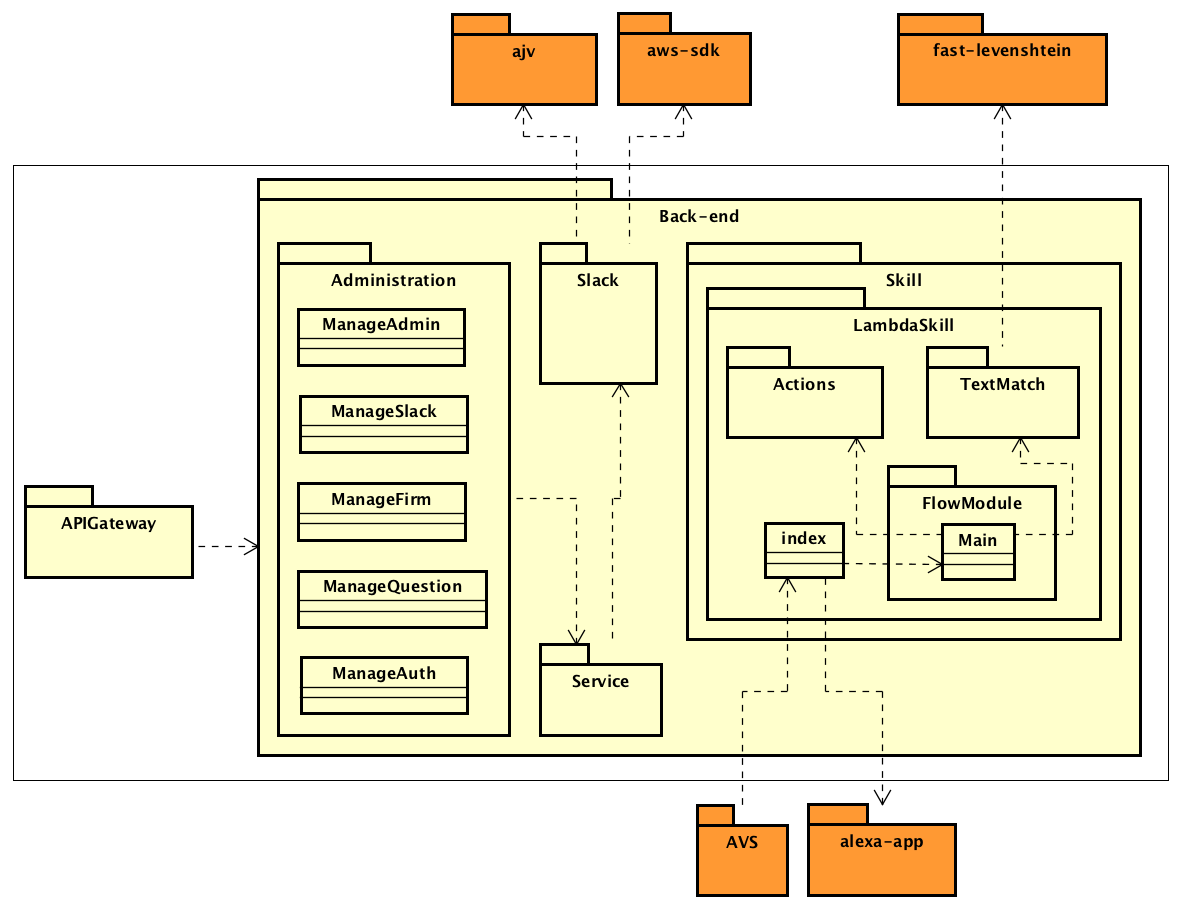
\includegraphics[width=\textwidth]{Architettura/Back-end.png}
	\caption{Schema del componente \texttt{Back-End}}
\end{figure}
\paragraph{Informazioni sul package}\begin{itemize}\item \textbf{Descrizione}: Package che contiene tutti i package dedicati alla parte logica dell'applicazione\item \textbf{Package contenuti}:
	\begin{itemize}\item Back-End :: Action: Package che contiene le possibili azioni in risposta alle interazioni
	\item Back-End :: Administration: Package che contiene tutte le funzionalità che un Admin ed un SuperAdmin possono avere
	\item Back-End :: DatabaseInteraction: package per la gestione del database
	\item Back-End :: Interaction: package per il tramite tra APIGateway e AVS
	\item Back-End :: Service: Package che gestisce tutti i servizi disponibili nell'applicazione
	\item Back-End :: Slack: package per la gestione di Slack
	\end{itemize}\end{itemize}

	\newpage
	\subsubsection{ \texttt{Back-End :: Action}}
	\paragraph{Informazioni sul package}


	\begin{itemize}\item \textbf{Descrizione}: Package che contiene le possibili azioni in risposta alle interazioni.\\
	La classe contenuta in questo package non è ancora stata ben definita, poichè un inserimento più ampio di azioni è previsto come requisito opzionale, quindi la definizione specifica di questa classe viene rimandata dopo la codifica dei requisiti obbligatori.  \item \textbf{Padre}: Back-End\paragraph{Classi}
	\subparagraph{\texttt{Back-End :: Action :: Actions}}
	\begin{itemize}\item \textbf{Descrizione}: Classe che contiene tutti i metodi che forniscono azioni predefinite
	\item \textbf{Utilizzo}: Verrà utilizzata per contenere tutti i metodi per le ACTION predefinite nel sistema
	\item \textbf{Relazioni con altre classi}:
	\begin{itemize}
	\item \texttt{Back-End :: Service :: FirmService}: Classe che implementa i servizi dedicati alla gestione del Firm di un azienda;
	\item \texttt{Back-End :: Service :: QuestionService}: Fornisce i servizi per gestione delle domande.;
	\item \texttt{Back-End :: Service :: SlackService}: Classe che implementa i metodi forniti dalla classe Interlocutor e fornisce servizi specifici per la gestione del canale \#azienda.
	\end{itemize}
	\end{itemize}\end{itemize}

	\newpage
	\subsubsection{ \texttt{Back-End :: Administration}}
	\begin{figure}[!h]
		\centering
		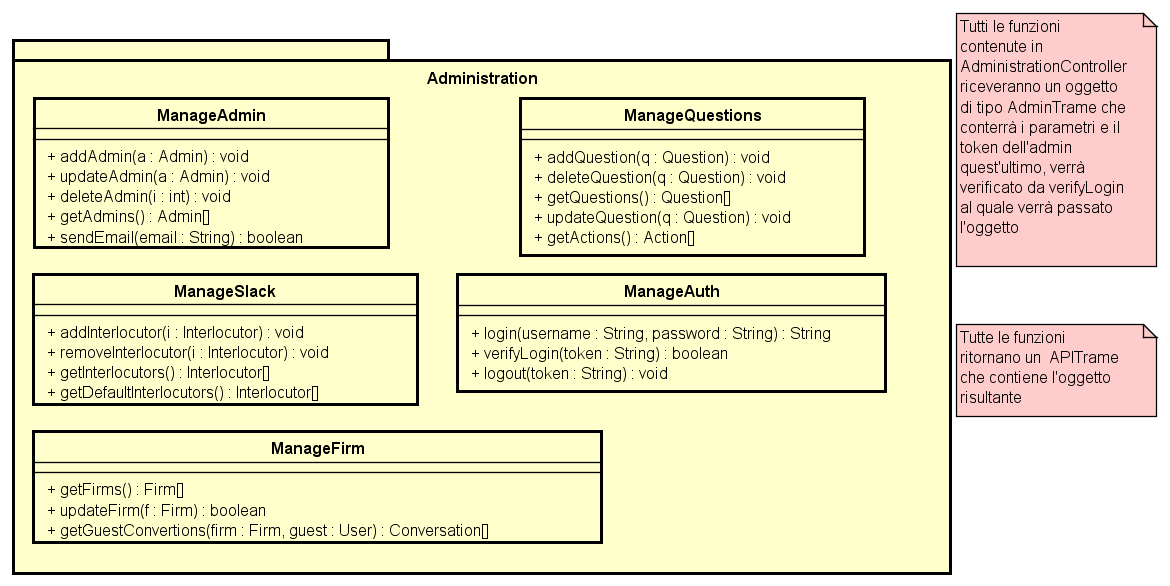
\includegraphics[width=\textwidth]{Architettura/Back-End/Administration.png}
		\caption{Schema del componente \texttt{Back-End :: Administration}}
	\end{figure}
	\paragraph{Informazioni sul package}\begin{itemize}\item \textbf{Descrizione}: Package che contiene tutte le funzionalità che un Admin ed un SuperAdmin possono avere\item \textbf{Padre}: Back-End\paragraph{Classi}
	\subparagraph{\texttt{Back-End :: Administration :: ManageAdmin}}
	\begin{itemize}\item \textbf{Descrizione}: Classe utilizzata per la gestione degli amministratori
	\item \textbf{Utilizzo}: gestione amministratori
	\item \textbf{Metodi}:
	\begin{itemize}
	\item \texttt{addAdmin(a) : void}\

	 Metodo che aggiunge un Admin all'array di Admin

	\item \textbf{Argomenti}:
	\begin{itemize}
	\item \texttt{a : Admin}\

	 Parametro che rappresenta l'oggetto ti tipo Admin che si vuole agiungere.
	\end{itemize}
	\end{itemize}\vspace{0.5em}
	\begin{itemize}
	\item \texttt{deleteAdmin(i) : void}\

	 Metodo che permette di eliminare un Admin dall'array degli Admin

	\item \textbf{Argomenti}:
	\begin{itemize}
	\item \texttt{i : int}\

	 Parametro intero che indica l'i-simo Admin che verrà eliminato dall'array di Admin.
	\end{itemize}
	\end{itemize}\vspace{0.5em}
	\begin{itemize}
	\item \texttt{getAdmins() : Admin[]}\

	 Metodo che restituisce l'intero array di Admin
	\end{itemize}\vspace{0.5em}
	\begin{itemize}
	\item \texttt{sendEmail(email) : boolean}\

	 Metodo che spedisce una e-mail all'indirizzo specificato

	\item \textbf{Argomenti}:
	\begin{itemize}
	\item \texttt{email : string}\

	 Parametro stringa che specifica l'indirizzo desiderato per l'e-mail.
	\end{itemize}
	\end{itemize}\vspace{0.5em}
	\begin{itemize}
	\item \texttt{updateAdmin(a) : void}\

	 Metodo che aggiorna un Admin

	\item \textbf{Argomenti}:
	\begin{itemize}
	\item \texttt{a : Admin}\

	 Parametro che rappresenta l'oggetto di tipo Admin da modificare.
	\end{itemize}
	\end{itemize}\vspace{0.5em}
	\item \textbf{Relazioni con altre classi}:
	\begin{itemize}
	\item \texttt{Back-End :: Service :: AdminService}: Classe che fornisce dei servizi specifici per gli Admin ed i SuperAdmin.
	\end{itemize}
	\end{itemize}\subparagraph{\texttt{Back-End :: Administration :: ManageAuth}}
	\begin{itemize}\item \textbf{Descrizione}: Classe adibita ai permessi di autenticazione
	\item \textbf{Utilizzo}: Classe utilizzata per autenticare l'Admin ed il SuperAdmin
	\item \textbf{Metodi}:
	\begin{itemize}
	\item \texttt{login(username) : string}\

	 Effettua l'operazione di login ritornando un token relativo a quella sessione.

	\item \textbf{Argomenti}:
	\begin{itemize}
	\item \texttt{username : string}\

	 Nome utente di cui sarà effettuata la login.
	\end{itemize}
	\end{itemize}\vspace{0.5em}
	\begin{itemize}
	\item \texttt{logout(token) : void}\

	 Chiude la sessione attiva utilizzando il token generato dall'operazione di login.

	\item \textbf{Argomenti}:
	\begin{itemize}
	\item \texttt{token : string}\

	 stringa generata dall'operazione di login.
	\end{itemize}
	\end{itemize}\vspace{0.5em}
	\begin{itemize}
	\item \texttt{verifyAdminTrame(trame) : void}\

	 Verifica che il trame passato in ingresso sia corretto e, nel caso si verificasse un errore, verrà lanciata un eccezione.

	\item \textbf{Argomenti}:
	\begin{itemize}
	\item \texttt{trame : AdminTrame}\

	 Contiene il trame relativo ad un Admin.
	\end{itemize}
	\end{itemize}\vspace{0.5em}
	\begin{itemize}
	\item \texttt{verifyLogin(token) : boolean}\

	 Verifica della sessione attiva tramite il token generato dall'operazione di login(username:string,password:string).

	\item \textbf{Argomenti}:
	\begin{itemize}
	\item \texttt{token : string}\

	 Contiene la stringa generata alla creazione della login.
	\end{itemize}
	\end{itemize}\vspace{0.5em}
	\item \textbf{Relazioni con altre classi}:
	\begin{itemize}
	\item \texttt{Back-End :: Service :: AdminService}: Classe che fornisce dei servizi specifici per gli Admin ed i SuperAdmin.
	\end{itemize}
	\end{itemize}\subparagraph{\texttt{Back-End :: Administration :: ManageFirm}}
	\begin{itemize}\item \textbf{Descrizione}: Classe utilizzata per la gestione delle aziende
	\item \textbf{Utilizzo}: gestione aziende
	\item \textbf{Metodi}:
	\begin{itemize}
	\item \texttt{getFirm() : Firm[]}\

	 Restituisce un array di oggetti di tipo Firm con i nomi delle aziende
	\end{itemize}\vspace{0.5em}
	\begin{itemize}
	\item \texttt{getGuestConvertions(f, User) : Conversation[]}\

	 Ritorna un array con le conversazioni di un ospite di un'azienda

	\item \textbf{Argomenti}:
	\begin{itemize}
	\item \texttt{f : Firm}\

	 Contiene un oggetto di tipo Firm.
	\item \texttt{User : Guest}\

	 Contiene l'ospite che ha effettuato la conversazione.
	\end{itemize}
	\end{itemize}\vspace{0.5em}
	\begin{itemize}
	\item \texttt{updateFirm(f) : boolean}\

	 Aggiunta di una firma e ritorno se l'operazione ha avuto successo.

	\item \textbf{Argomenti}:
	\begin{itemize}
	\item \texttt{f : Firm}\

	 Contiene un oggetto di tipo Firm.
	\end{itemize}
	\end{itemize}\vspace{0.5em}
	\item \textbf{Relazioni con altre classi}:
	\begin{itemize}
	\item \texttt{Back-End :: Service :: AdminService}: Classe che fornisce dei servizi specifici per gli Admin ed i SuperAdmin;
	\item \texttt{Back-End :: Service :: FirmService}: Classe che implementa i servizi dedicati alla gestione dell'oggetto di tipo Firm.
	\end{itemize}
	\end{itemize}\subparagraph{\texttt{Back-End :: Administration :: ManageQuestion}}
	\begin{itemize}\item \textbf{Descrizione}: Classe utilizzata per modificare le domande e visionare le azioni associate
	\item \textbf{Utilizzo}: Classe utilizzata quando si vuole manipolare in generale l'array delle domande
	\item \textbf{Attributi}:
	\begin{itemize}
	\item \texttt{-API\_PATH: JSONObject}\

	 Attributo che rappresenta il percorso per le API in formato JSON.
	\end{itemize}
	\begin{itemize}
	\item \texttt{-http: Module}\

	 Attributo che rappresenta il modulo per la connessione http.
	\end{itemize}
	\begin{itemize}
	\item \texttt{-token: string}\

	 Stringa che contiene il token.
	\end{itemize}
	\item \textbf{Metodi}:
	\begin{itemize}
	\item \texttt{addQuestion(q) : void}\

	 Metodo per aggiungere una domanda all'array Question[] delle domande.

	\item \textbf{Argomenti}:
	\begin{itemize}
	\item \texttt{q : Question}\

	 Parametro che indica l'oggetto di tipo Question che si vuole aggiungere all'array delle domande.
	\end{itemize}
	\end{itemize}\vspace{0.5em}
	\begin{itemize}
	\item \texttt{deleteQuestion(q) : void}\

	 Metodo per eliminare una domanda dall'array delle domande.

	\item \textbf{Argomenti}:
	\begin{itemize}
	\item \texttt{q : Question}\

	 Parametro che indica quale oggetto di tipo Question si vuole eliminare dall'array delle domande.
	\end{itemize}
	\end{itemize}\vspace{0.5em}
	\begin{itemize}
	\item \texttt{getActions() : Action[]}\

	 Metodo che restituisce l'intero array delle azioni disponibili
	\end{itemize}\vspace{0.5em}
	\begin{itemize}
	\item \texttt{getQuestions() : Question[]}\

	 Metodo che ritorna l'intero array delle domande
	\end{itemize}\vspace{0.5em}
	\begin{itemize}
	\item \texttt{updateQuestion(q) : void}\

	 Metodo che aggiorna una domanda nell'array delle domande

	\item \textbf{Argomenti}:
	\begin{itemize}
	\item \texttt{q : Question}\

	 Parametro che indica quale oggetto di tipo Question si vuole modificare.
	\end{itemize}
	\end{itemize}\vspace{0.5em}
	\item \textbf{Relazioni con altre classi}:
	\begin{itemize}
	\item \texttt{Back-End :: Service :: AdminService}: Classe che fornisce dei servizi specifici per gli Admin ed i SuperAdmin;
	\item \texttt{Back-End :: Service :: QuestionService}: Fornisce i servizi per gestione delle domande.
	\end{itemize}
	\end{itemize}\subparagraph{\texttt{Back-End :: Administration :: ManageSlack}}
	\begin{itemize}\item \textbf{Descrizione}: Classe utilizzata per la gestione di Slack
	\item \textbf{Utilizzo}: gestione Slack
	\item \textbf{Metodi}:
	\begin{itemize}
	\item \texttt{addInterlocutor(interlocutor) : void}\

	 Aggiunge un interlocutore alla lista degli interlocutori possibili

	\item \textbf{Argomenti}:
	\begin{itemize}
	\item \texttt{interlocutor : Interlocutor}\

	 interlocutore da aggiungere nella lista di interlocutori.
	\end{itemize}
	\end{itemize}\vspace{0.5em}
	\begin{itemize}
	\item \texttt{getDefaultInterlocutors() : Interlocutor[]}\

	 Ritorna un array di tutti gli interlocutori che sono inseriti di default, in ascolto in un canale aziendale nuovo, presenti nel database
	\end{itemize}\vspace{0.5em}
	\begin{itemize}
	\item \texttt{getInterlocutors() : Interlocutor[]}\

	 Ritorna un array di tutti gli interlocutori presenti nel database
	\end{itemize}\vspace{0.5em}
	\begin{itemize}
	\item \texttt{removeInterlocutor(interlocutor) : void}\

	 Rimuove l'interlocutore passato come parametro

	\item \textbf{Argomenti}:
	\begin{itemize}
	\item \texttt{interlocutor : Interlocutor}\

	 Contiene l'interlocutore che sarà successivamente eliminato dalla lista degli interlocutori di Slack.
	\end{itemize}
	\end{itemize}\vspace{0.5em}
	\item \textbf{Relazioni con altre classi}:
	\begin{itemize}
	\item \texttt{Back-End :: Service :: AdminService}: Classe che fornisce dei servizi specifici per gli Admin ed i SuperAdmin;
	\item \texttt{Back-End :: Slack :: Slack}: Classe utilizzata per la gestione degli ospiti su Slack.
	\end{itemize}
	\end{itemize}\end{itemize}

	\newpage
	\subsubsection{ \texttt{Back-End :: DatabaseInteraction}}
	\begin{figure}[!h]
		\centering
		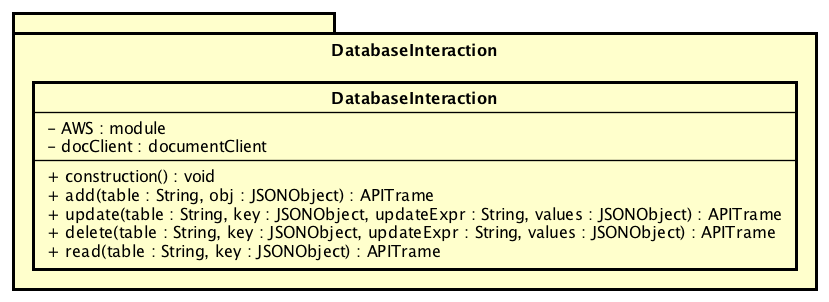
\includegraphics[scale=0.7]{Architettura/Back-End/DatabaseInteraction.png}
		\caption{Schema del componente \texttt{Back-End :: DatabaseInteraction}}
	\end{figure}
	\paragraph{Informazioni sul package}\begin{itemize}\item \textbf{Descrizione}: package per la gestione del database\item \textbf{Padre}: Back-End\paragraph{Classi}
	\subparagraph{\texttt{Back-End :: DatabaseInteraction :: DatabaseInteraction}}
	\begin{itemize}\item \textbf{Descrizione}: Classe che si occupa della connessione con il database e delle operazioni di lettura e scrittura.
	\item \textbf{Utilizzo}: Utilizzata per operazioni di lettura e scrittura nel database.
	\item \textbf{Attributi}:
	\begin{itemize}
	\item \texttt{-AWS: Module}\

	 Modulo importato da Amazon per interagire con AWS.
	\end{itemize}
	\begin{itemize}
	\item \texttt{-docClient: documentClient}\

	 Oggetto derivato da AWS-SDK.
	\end{itemize}
	\item \textbf{Metodi}:
	\begin{itemize}
	\item \texttt{add(obj, table) : APITrame}\

	 Inserisce un nuovo JSONObject. Il tipo di ritorno APITrame è necessario per controllare se c'è un errore nell'operazione.

	\item \textbf{Argomenti}:
	\begin{itemize}
	\item \texttt{obj : JSONObject}\

	 Contiene l'oggetto JSON da inserire nel database.
	\item \texttt{table : string}\

	 Contiene la posizione, sulla quale inserire l'oggetto JSON, sotto forma di stringa.
	\end{itemize}
	\end{itemize}\vspace{0.5em}
	\begin{itemize}
	\item \texttt{construction() : void}\

	 Crea il l'oggetto DatabaseInteraction.
	\end{itemize}\vspace{0.5em}
	\begin{itemize}
	\item \texttt{delete(key, table, updatExpr, values) : JSONObject}\

	 Metodo per eliminare i campi del database. Il tipo di ritorno APITrame è necessario per controllare se c'è un errore nell'operazione.


	\item \textbf{Argomenti}:
	\begin{itemize}
	\item \texttt{key : JSONObject}\

	 Rappresenta la chiave utilizzata nel db.
	\item \texttt{table : string}\

	 Nome della tabella, utilizzato come percorso.
	\item \texttt{updatExpr : string}\

	 Caratteristiche da trovare e modificare, rappresenta la condizione.
	\item \texttt{values : JSONObject}\

	 Valore richiesto come parametro in input.
	\end{itemize}
	\end{itemize}\vspace{0.5em}
	\begin{itemize}
	\item \texttt{read(key, text) : APITrame}\

	 Ricerca nella collezione con i criteri passati.

	\item \textbf{Argomenti}:
	\begin{itemize}
	\item \texttt{key : JSONObject}\

	 Rappresenta la chiave utilizzata nel db.
	\item \texttt{text : string}\

	 Nome della tabella, utilizzato come percorso.
	\end{itemize}
	\end{itemize}\vspace{0.5em}
	\begin{itemize}
	\item \texttt{update(key, table, updateExpr, values) : APITrame}\

	 Metodo per aggiornare i campi del database. Il tipo di ritorno APITrame è necessario per controllare se c'è un errore nell'operazione.

	\item \textbf{Argomenti}:
	\begin{itemize}
	\item \texttt{key : JSONObject}\

	 Rappresenta la chiave utilizzata nel db.
	\item \texttt{table : string}\

	 Rappresenta il nome della tabella utilizzato come percorso.
	\item \texttt{updateExpr : string}\

	 Caratteristiche da trovare e modificare, rappresenta la condizione.
	\item \texttt{values : JSONObject}\

	 Nuovo valore da inserire.
	\end{itemize}
	\end{itemize}\vspace{0.5em}
	\end{itemize}\end{itemize}

	\newpage
	\subsubsection{ \texttt{Back-End :: Interaction}}
	\begin{figure}[!h]
		\centering
		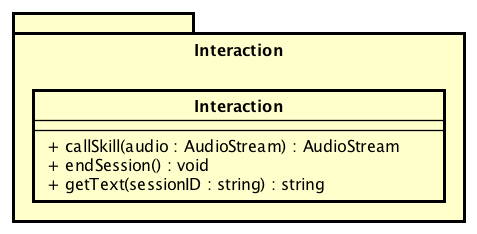
\includegraphics[scale=0.7]{Architettura/Back-End/Interaction.png}
		\caption{Schema del componente \texttt{Back-End :: Interaction}}
	\end{figure}
	\paragraph{Informazioni sul package}\begin{itemize}\item \textbf{Descrizione}: package per il tramite tra APIGateway e AVS\item \textbf{Padre}: Back-End\paragraph{Classi}
	\subparagraph{\texttt{Back-End :: Interaction :: Interaction}}
	\begin{itemize}\item \textbf{Descrizione}: Classe utilizzata per la gestione dell'interazione tra APIGateway e AVS
	\item \textbf{Utilizzo}: gestione interazione
	\item \textbf{Metodi}:
	\begin{itemize}
	\item \texttt{callSkill(audio) : AudioStream}\

	 Metodo per chiamare la skill a cui passare la risposta dell'ospite

	\item \textbf{Argomenti}:
	\begin{itemize}
	\item \texttt{audio : AudioStream}\

	 Risposta dell'ospite.
	\end{itemize}
	\end{itemize}\vspace{0.5em}
	\begin{itemize}
	\item \texttt{endSession() : void}\

	 Metodo per terminare la sessione in corso
	\end{itemize}\vspace{0.5em}
	\begin{itemize}
	\item \texttt{getText(sessionID) : string}\

	 Metodo per avere il testo dell'ultima risposta data dall'ospite

	\item \textbf{Argomenti}:
	\begin{itemize}
	\item \texttt{sessionID : string}\

	 ID della sessione a cui richiedere il testo della risposta.
	\end{itemize}
	\end{itemize}\vspace{0.5em}
	\end{itemize}\end{itemize}

	\newpage
	\subsubsection{ \texttt{Back-End :: Service}}
	\begin{figure}[!h]
		\centering
		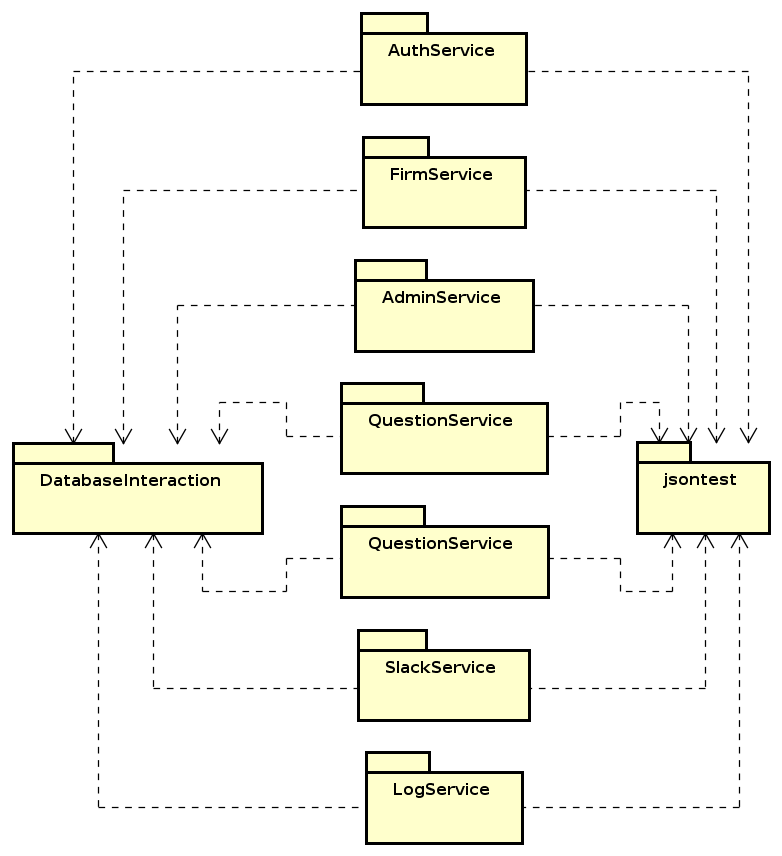
\includegraphics[width=\textwidth]{Architettura/Back-End/Service.png}
		\caption{Schema del componente \texttt{Back-End :: Service}}
	\end{figure}
	\paragraph{Informazioni sul package}\begin{itemize}\item \textbf{Descrizione}: Package che gestisce tutti i servizi disponibili nell'applicazione\item \textbf{Padre}: Back-End\paragraph{Classi}
	\subparagraph{\texttt{Back-End :: Service :: AdminService}}
	\begin{itemize}\item \textbf{Descrizione}: Classe che fornisce dei servizi specifici per gli Admin ed i SuperAdmin
	\item \textbf{Utilizzo}: Classe utilizzata quando viene chiamato un servizio disponibile per Admin e SuperAdmin
	\item \textbf{Metodi}:
	\begin{itemize}
	\item \texttt{addAdmin(admin) : void}\

	 Metodo che aggiunge un Admin nell'array degli Admin

	\item \textbf{Argomenti}:
	\begin{itemize}
	\item \texttt{admin : Admin}\

	 Parametro che indica l'oggetto di tipo Admin che si vuole aggiungere.
	\end{itemize}
	\end{itemize}\vspace{0.5em}
	\begin{itemize}
	\item \texttt{deleteAdmin(admin) : void}\

	 Metodo che elimina un Admin dall'array degli Admin

	\item \textbf{Argomenti}:
	\begin{itemize}
	\item \texttt{admin : Admin}\

	 Parametro che indica quale oggetto di tipo Admin si vuole eliminare.
	\end{itemize}
	\end{itemize}\vspace{0.5em}
	\begin{itemize}
	\item \texttt{getAdmins() : Admin[]}\

	 Metodo che restituisce l'intero array degli Admin
	\end{itemize}\vspace{0.5em}
	\begin{itemize}
	\item \texttt{login(password, username) : string}\

	 Metodo che effettua l'operazione di login ritornando un token relativo a quella sessione.

	\item \textbf{Argomenti}:
	\begin{itemize}
	\item \texttt{password : string}\

	 Parametro che rappresenta la password dell'ospite che intende effettuare la login.
	\item \texttt{username : string}\

	 Parametro che rappresenta l'username dell'ospite che vuole effettuare il login.
	\end{itemize}
	\end{itemize}\vspace{0.5em}
	\begin{itemize}
	\item \texttt{logout(token) : void}\

	 Metodo che chiude la sessione attiva utilizzando il token generato dall'operazione di login.

	\item \textbf{Argomenti}:
	\begin{itemize}
	\item \texttt{token : string}\

	 Parametro che rappresenta il token dell'Admin di cui si vuole terminare la sessione.
	\end{itemize}
	\end{itemize}\vspace{0.5em}
	\begin{itemize}
	\item \texttt{sendEmail(at) : void}\

	 Invia la mail per il recupero della password all'indirizzo passato tramite stringa.

	\item \textbf{Argomenti}:
	\begin{itemize}
	\item \texttt{at : AdminTrame}\

	 Parametro che rappresenta l'oggetto JSON da verificare con lo schema. .
	\end{itemize}
	\end{itemize}\vspace{0.5em}
	\begin{itemize}
	\item \texttt{updateAdmin(admin) : void}\

	 Metodo che aggiorna un Admin

	\item \textbf{Argomenti}:
	\begin{itemize}
	\item \texttt{admin : Admin}\

	 Parametro che indica quale oggetto di tipo Admin si vuole aggiornare.
	\end{itemize}
	\end{itemize}\vspace{0.5em}
	\begin{itemize}
	\item \texttt{verifyLogin(token) : boolean}\

	 Metodo che verifica della sessione attiva tramite il token generato dall'operazione di login(username:string,password:string).

	\item \textbf{Argomenti}:
	\begin{itemize}
	\item \texttt{token : string}\

	 Parametro che contiene la stringa generata alla creazione della login.
	\end{itemize}
	\end{itemize}\vspace{0.5em}
	\end{itemize}\subparagraph{\texttt{Back-End :: Service :: FirmService}}
	\begin{itemize}\item \textbf{Descrizione}: Classe che implementa i servizi dedicati alla gestione di un oggetto di tipo Firm
	\item \textbf{Utilizzo}: Gestione di un oggetto di tipo Firm
	\item \textbf{Metodi}:
	\begin{itemize}
	\item \texttt{addInteraction(answerText, questionText, sessionID) : void}\

	 Aggiunge un interazione al Log.

	\item \textbf{Argomenti}:
	\begin{itemize}
	\item \texttt{answerText : string}\

	 Contiene il testo dell'ultima risposta data.
	\item \texttt{questionText : string}\

	 Contiene il testo di una domanda.
	\item \texttt{sessionID : string}\

	 Contiene il token relativo alla sessione.
	\end{itemize}
	\end{itemize}\vspace{0.5em}
	\begin{itemize}
	\item \texttt{getFirms() : Firm[]}\

	 Restituisce l'array con gli oggetti di tipo Firm presenti.
	\end{itemize}\vspace{0.5em}
	\begin{itemize}
	\item \texttt{getGuestConversation(firm, guest) : Conversation[]}\

	 Funzione che permette di ottenere le conversazioni di un ospite.

	\item \textbf{Argomenti}:
	\begin{itemize}
	\item \texttt{firm : Firm}\

	 Rappresenta l'azienda di appartenenza dell'ospite.
	\item \texttt{guest : User}\

	 Contiene i dati dell'ospite di cui sarà controllata la presenza del database.
	\end{itemize}
	\end{itemize}\vspace{0.5em}
	\begin{itemize}
	\item \texttt{isGuestPresent(name) : boolean}\

	 Controlla la presenza di un ospite all'interno del database.

	\item \textbf{Argomenti}:
	\begin{itemize}
	\item \texttt{name : string}\

	 Contiene il nome di un ospite.
	\end{itemize}
	\end{itemize}\vspace{0.5em}
	\begin{itemize}
	\item \texttt{isPresent(name) : boolean}\

	 Metodo che controlla l'esistenza di un'azienda con il nome passato.

	\item \textbf{Argomenti}:
	\begin{itemize}
	\item \texttt{name : string}\

	 Nome dell'azienda.
	\end{itemize}
	\end{itemize}\vspace{0.5em}
	\begin{itemize}
	\item \texttt{updateFirm(firm) : void}\

	 Metodo per l'inserimento di nuova azienda all'interno del database.

	\item \textbf{Argomenti}:
	\begin{itemize}
	\item \texttt{firm : Firm}\

	 Contiene un oggetto di tipo Firm.
	\end{itemize}
	\end{itemize}\vspace{0.5em}
	\end{itemize}\subparagraph{\texttt{Back-End :: Service :: QuestionService}}
	\begin{itemize}\item \textbf{Descrizione}: Fornisce i servizi per gestione delle domande.
	\item \textbf{Utilizzo}: Usato per le chiamate relative ai servizi di gestione delle domande.
	\item \textbf{Metodi}:
	\begin{itemize}
	\item \texttt{addQuestion(question) : void}\

	 Questo metodo fornisce il servizio per l'aggiunta di una domanda.

	\item \textbf{Argomenti}:
	\begin{itemize}
	\item \texttt{question : Question}\

	 Contiene una domanda da inserire nel database nella lista delle domande.
	\end{itemize}
	\end{itemize}\vspace{0.5em}
	\begin{itemize}
	\item \texttt{deleteQuestion(question) : void}\

	 Metodo che permette di eliminare una domanda precedentemente inserita.

	\item \textbf{Argomenti}:
	\begin{itemize}
	\item \texttt{question : Question}\

	 Contiene tutte le informazioni relative ad una domanda.
	\end{itemize}
	\end{itemize}\vspace{0.5em}
	\begin{itemize}
	\item \texttt{getActions() : Action[]}\

	 Restituisce un array contenente tutte le azioni possibili in risposta alle interazioni.
	\end{itemize}\vspace{0.5em}
	\begin{itemize}
	\item \texttt{getNextQuestion(anction) : Question}\

	 Restituisce la domanda successiva usando in ingresso la risposta data, con tutte le relative informazioni.

	\item \textbf{Argomenti}:
	\begin{itemize}
	\item \texttt{anction : Action}\

	 Contiene tutte le informazioni relative ad una risposta data.
	\end{itemize}
	\end{itemize}\vspace{0.5em}
	\begin{itemize}
	\item \texttt{getQuestions(question) : Question[]}\

	 Restituisce un array di Question con tutte le domande presenti nel DB.

	\item \textbf{Argomenti}:
	\begin{itemize}
	\item \texttt{question : Question[]}\

	 Contiene tutte le informazioni relative ad una domanda.
	\end{itemize}
	\end{itemize}\vspace{0.5em}
	\begin{itemize}
	\item \texttt{updateQuestion(questionq) : void}\

	 Permette la modifica delle informazioni di una domanda.

	\item \textbf{Argomenti}:
	\begin{itemize}
	\item \texttt{questionq : Question}\

	 Contiene tutte le informazioni relative ad una domanda.
	\end{itemize}
	\end{itemize}\vspace{0.5em}
	\begin{itemize}
	\item \texttt{getFirstquestion() : Question}\

	 Chiamata iniziale che permette l'inizio delle interazioni successive restituendo la prima domanda.
	\end{itemize}\vspace{0.5em}
	\begin{itemize}
	\item \texttt{getLastAnswerText(skillSessionID) : string}\

	 Restituisce il testo dell'ultima risposta data nella conversazione.

	\item \textbf{Argomenti}:
	\begin{itemize}
	\item \texttt{skillSessionID : string}\

	 Contiene il token della sessione in corso.
	\end{itemize}
	\end{itemize}\vspace{0.5em}
	\end{itemize}\subparagraph{\texttt{Back-End :: Service :: SlackService}}
	\begin{itemize}\item \textbf{Descrizione}: Classe che implementa i metodi forniti dalla classe Interlocutor e fornisce servizi specifici per la gestione del canale \#azienda
	\item \textbf{Utilizzo}: Classe utilizzata quando viene chiamato un servizio disponibile per Admin e SuperAdmin
	\item \textbf{Metodi}:
	\begin{itemize}
	\item \texttt{refreshInterlocutors() : void}\

	 Metodo che aggiorna la lista degli interlocutori presenti nel database recuperandoli dalla lista degli interlocutori presenti nel canale Slack dell'azienda.
	\end{itemize}\vspace{0.5em}
	\begin{itemize}
	\item \texttt{sendMessageChannel(firmName, text) : void}\

	 Metodo che scrive un messaggio passato sotto forma di stringa nel canale che viene passato come stringa.

	\item \textbf{Argomenti}:
	\begin{itemize}
	\item \texttt{firmName : string}\

	 Parametro che rappresenta il nome del canale nel quale scrivere il messaggio.
	\item \texttt{text : string}\

	 Parametro che rappresenta il testo del messaggio da scrivere nel canale.
	\end{itemize}
	\end{itemize}\vspace{0.5em}
	\begin{itemize}
	\item \texttt{sendMessageGeneral(text) : void}\

	 Metodo che scrive un messaggio passato sotto forma di stringa nel canale \#General .

	\item \textbf{Argomenti}:
	\begin{itemize}
	\item \texttt{text : string}\

	 Parametro che rappresenta il messaggio da scrivere nel canale \#General.
	\end{itemize}
	\end{itemize}\vspace{0.5em}
	\begin{itemize}
	\item \texttt{addInterlocutor(interlocutor) : void}\

	 Metodo che associa un interlocutore alla lista di default degli interlocutori che verrà utilizzata nel canale \#azienda di Slack

	\item \textbf{Argomenti}:
	\begin{itemize}
	\item \texttt{interlocutor : Interlocutor}\

	 Parametro che indica l'interlocutore di tipo Interlocutor da aggiungere alla lista.
	\end{itemize}
	\end{itemize}\vspace{0.5em}
	\begin{itemize}
	\item \texttt{getDefaultInterlocutors() : Interlocutor[]}\

	 Metodo che ritorna tutti gli interlocutori presenti nella lista di default utilizzata nel canale \#azienda di Slack
	\end{itemize}\vspace{0.5em}
	\begin{itemize}
	\item \texttt{getInterlocutors() : Interlocutor[]}\

	 Metodo che ritorna tutti gli interlocutori presenti nel sistema
	\end{itemize}\vspace{0.5em}
	\begin{itemize}
	\item \texttt{removeInterlocutor(interlocutor) : void}\

	 Metodo che disassocia un interlocutore alla lista di default degli interlocutori che verrà utilizzata nel canale \#azienda di Slack

	\item \textbf{Argomenti}:
	\begin{itemize}
	\item \texttt{interlocutor : Interlocutor}\

	 Parametro che indica l'interlocutore di tipo Interlocutor da rimuovere dalla lista.
	\end{itemize}
	\end{itemize}\vspace{0.5em}
	\end{itemize}\end{itemize}

	\newpage
	\subsubsection{ \texttt{Back-End :: Slack}}
	\begin{figure}[!h]
		\centering
		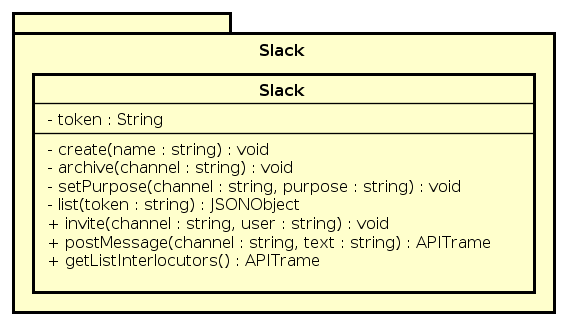
\includegraphics[scale=0.7]{Architettura/Back-End/Slack.png}
		\caption{Schema del componente \texttt{Back-End :: Slack}}
	\end{figure}
	\paragraph{Informazioni sul package}\begin{itemize}\item \textbf{Descrizione}: package per la gestione di Slack\item \textbf{Padre}: Back-End\paragraph{Classi}
	\subparagraph{\texttt{Back-End :: Slack :: Slack}}
	\begin{itemize}\item \textbf{Descrizione}: Classe utilizzata per la gestione degli ospiti su Slack
	\item \textbf{Utilizzo}: ospiti in Slack
	\item \textbf{Attributi}:
	\begin{itemize}
	\item \texttt{-token: string}\

	 Identificativo univoco del bot di Slack che viene utilizzato per il riconoscimento.
	\end{itemize}
	\item \textbf{Metodi}:
	\begin{itemize}
	\item \texttt{getListInterlocutors() : APITrame}\

	 Restituisce la lista di interlocutori utilizzando anche il metodo list.
	\end{itemize}\vspace{0.5em}
	\begin{itemize}
	\item \texttt{invite(channel, user) : void}\

	 Aggiunge un interlocutore al canale.

	\item \textbf{Argomenti}:
	\begin{itemize}
	\item \texttt{channel : string}\

	 Canale Slack.
	\item \texttt{user : string}\

	 Interlocutore del canale.
	\end{itemize}
	\end{itemize}\vspace{0.5em}
	\begin{itemize}
	\item \texttt{postMessage(channel, Text) : APITrame}\

	 Invia un nuovo messaggio Slack.

	\item \textbf{Argomenti}:
	\begin{itemize}
	\item \texttt{channel : string}\

	 Nome del canale.
	\item \texttt{Text : string}\

	 Testo del messaggio.
	\end{itemize}
	\end{itemize}\vspace{0.5em}
	\begin{itemize}
	\item \texttt{archive(channel) : void}\

	 Chiama il metodo di Slack per l'archiviazione del canale.

	\item \textbf{Argomenti}:
	\begin{itemize}
	\item \texttt{channel : string}\

	 Canale di Slack.
	\end{itemize}
	\end{itemize}\vspace{0.5em}
	\begin{itemize}
	\item \texttt{create(name) : void}\

	 Crea un nuovo canale per l'ospite.

	\item \textbf{Argomenti}:
	\begin{itemize}
	\item \texttt{name : string}\

	 Nome del canale per l'ospite.
	\end{itemize}
	\end{itemize}\vspace{0.5em}
	\begin{itemize}
	\item \texttt{list() : JSONObject}\

	 Restituisce un oggetto JSONObject con tutti gli utenti Slack del canale.
	\end{itemize}\vspace{0.5em}
	\begin{itemize}
	\item \texttt{setPurpose(channel) : void}\

	 Metodo per il settaggio dello scopo del canale su Slack.

	\item \textbf{Argomenti}:
	\begin{itemize}
	\item \texttt{channel : string}\

	 Canale Slack.
	\end{itemize}
	\end{itemize}\vspace{0.5em}
	\end{itemize}\end{itemize}

	\newpage
	\subsubsection{ \texttt{LambdaSkill}}
	\begin{figure}[!h]
		\centering
		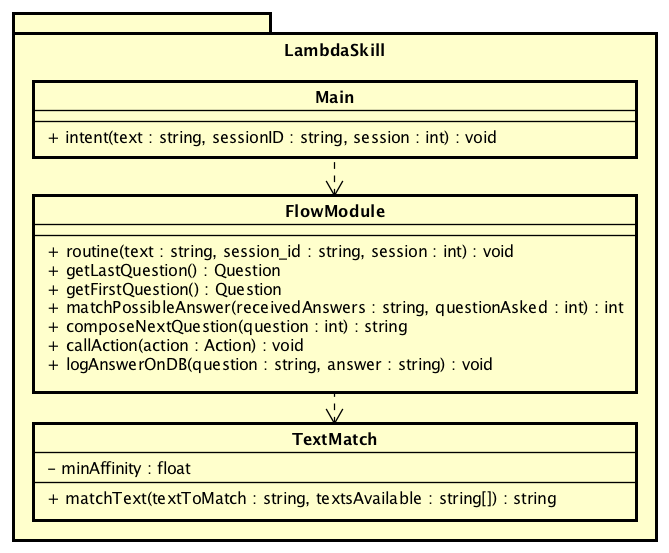
\includegraphics[scale=0.7]{Architettura/Back-End/LambdaSkill.png}
		\caption{Schema del componente \texttt{Back-End :: LambdaSkill}}
	\end{figure}
	\paragraph{Informazioni sul package}\begin{itemize}\item \textbf{Descrizione}: Package contenente la logica del workflow dell'applicazione
	\paragraph{Classi}
	\subparagraph{\texttt{Back-End :: LambdaSkill :: FlowModule}}
	\begin{itemize}\item \textbf{Descrizione}: Classe che viene usata per gestire l'intero work-flow della conversazione, quindi domande e risposte, tra l'AV e l'ospite
	\item \textbf{Utilizzo}: Sarà utilizzata per implementare la gestione delle conversazioni
	\item \textbf{Metodi}:
	\begin{itemize}
	\item \texttt{callAction(action) : void}\

	 Funzione che in base all'oggetto di tipo Action passato come parametro invoca la funzione hard coded corretta fra quelli predefinite

	\item \textbf{Argomenti}:
	\begin{itemize}
	\item \texttt{action : Action}\

	 Parametro che indica l'oggetto Action associato ad una funzione presente nel codice in maniera hard coded.
	\end{itemize}
	\end{itemize}\vspace{0.5em}
	\begin{itemize}
	\item \texttt{composeNextQuestion(question) : string}\

	 Funzione che identifica e ritorna la successiva domanda da porre all'utente come stringa


	\item \textbf{Argomenti}:
	\begin{itemize}
	\item \texttt{question : int}\

	 Parametro che indica l'id della precedente domanda effettuata all'utente.
	\end{itemize}
	\end{itemize}\vspace{0.5em}
	\begin{itemize}
	\item \texttt{getFirstQuestion() : Question}\

	 Funzione usata per ottenere la prima domanda da effettuare all'ospite

	\end{itemize}\vspace{0.5em}
	\begin{itemize}
	\item \texttt{getLastQuestion() : Question}\

	 Funzione usata per ottenere l'ultima domanda effettuata all'ospite
	\end{itemize}\vspace{0.5em}
	\begin{itemize}
	\item \texttt{logAnswerOnDB(answer, question) : void}\

	 Funzione che salva correttamente all'interno del database la coppia domanda-risposta in modo da mantenere un log delle conversazioni

	\item \textbf{Argomenti}:
	\begin{itemize}
	\item \texttt{answer : string}\

	 Parametro che indica la risposta ricevuta dall'utente.
	\item \texttt{question : string}\

	 Parametro che indica la domanda posta all'utente.
	\end{itemize}
	\end{itemize}\vspace{0.5em}
	\begin{itemize}
	\item \texttt{matchPossibileAnswer(questionAsked, receivedAnswer) : string}\

	 Funzione che identifica e ritorna il valore intero che rappresenta la risposta dell'utente, fra le possibili risposte ammesse dal nostro sistema

	\item \textbf{Argomenti}:
	\begin{itemize}
	\item \texttt{questionAsked : int}\

	 Parametro che indica l'id della risposta effettuata all'utente.
	\item \texttt{receivedAnswer : string}\

	 Parametro che indica la risposta inviata dall'utente e ricevuto dall'AV.
	\end{itemize}
	\end{itemize}\vspace{0.5em}
	\begin{itemize}
	\item \texttt{routine(session\_id) : void}\

	 Funzione usata per decodificare la stringa passata come parametro e, in base alla informazioni in essa contenute, chiamare altri metodi

	\item \textbf{Argomenti}:
	\begin{itemize}
	\item \texttt{session\_id : string}\

	 Parametro che indica l'id della sessione attiva.
	\end{itemize}
	\end{itemize}\vspace{0.5em}
	\item \textbf{Relazioni con altre classi}:
	\begin{itemize}
	\item \texttt{Back-End :: Service :: QuestionService}: Fornisce i servizi per gestione delle domande.;
	\item \texttt{Back-End :: LambdaSkill :: TextMatch}: Classe per verificare il grado di affinità tra la risposta dell'ospite e quelle accettate.
	\end{itemize}
	\end{itemize}\subparagraph{\texttt{Back-End :: LambdaSkill :: Main}}
	\begin{itemize}\item \textbf{Descrizione}: Classe utilizzata per gestire l'handler della Lambda function
	\item \textbf{Utilizzo}: Gestione handler
	\item \textbf{Metodi}:
	\begin{itemize}
	\item \texttt{intent(session, sessionID, text) : void}\

	 Metodo per la chiamata del FlowModule, si occupa anche dell'intent della Lambda Skill.

	\item \textbf{Argomenti}:
	\begin{itemize}
	\item \texttt{session : Session}\

	 Contiene i dati della sessione.
	\item \texttt{sessionID : string}\

	 Contiene il token della sessione.
	\item \texttt{text : string}\

	 Testo per la Lambda Skill.
	\end{itemize}
	\end{itemize}\vspace{0.5em}
	\item \textbf{Relazioni con altre classi}:
	\begin{itemize}
	\item \texttt{Back-End :: LambdaSkill :: FlowModule}: Classe che viene usata per gestire l'intero work-flow della conversazione, quindi domande e risposte, tra l'AV e l'ospite.
	\end{itemize}
	\begin{itemize}\item \textbf{Descrizione}: Classe utilizzata per verificare il grado di affinità tra la risposta dell'ospite e quelle accettate
	\end{itemize}\subparagraph{\texttt{Back-End :: LambdaSkill :: TextMatch}}
	\item \textbf{Utilizzo}: Verifica affinità risposta ospite
	\item \textbf{Metodi}:
	\begin{itemize}
	\item \texttt{matchText(textsAvailable, textToMatch) : string}\

	 Metodo per verificare se la riposta data dall'ospite corrisponde ad una di quelle accettate

	\item \textbf{Argomenti}:
	\begin{itemize}
	\item \texttt{textsAvailable : string[]}\

	 Vettore contente le riposte accettabili.
	\item \texttt{textToMatch : string}\

	 Testo della riposta data dall'ospite.
	\end{itemize}
	\end{itemize}\vspace{0.5em}
	\end{itemize}\end{itemize}


\subsection{ \texttt{Skill}}
\paragraph{Informazioni sul package}\begin{itemize}\item \textbf{Descrizione}: Contiene la configurazione di Amazon Skill Kit.\paragraph{Classi}
	\subparagraph{\texttt{Skill :: Skill}}
	\begin{itemize}\item \textbf{Descrizione}: rappresenta la configurazione di Amazon Alexa Skill Kit per la nostra applicazione.
	\item \textbf{Utilizzo}: Gestione Skill
	\item \textbf{Relazioni con altre classi}:
	\begin{itemize}
	\item \texttt{Back-End :: Main}: .
	\end{itemize}
	\end{itemize}\end{itemize}


\subsection{ \texttt{AVS}}\paragraph{Informazioni sul package}\begin{itemize}\item \textbf{Descrizione}: Package che si riferisce al componente esterno AVS (Alexa Voice Service), il quale viene utilizzato all'interno dell'architettura\end{itemize}

\subsection{ \texttt{aws-sdk}}\paragraph{Informazioni sul package}\begin{itemize}\item \textbf{Descrizione}: Package che si riferisce al componente esterno aws-sdk (Amazon Web Services SDK), il quale viene utilizzato all'interno dell'architettura\end{itemize}




\end{document}
